\chapter{Constraining Warm Dark Matter at the density level}\label{sec: inference pipeline}


\section{Inference pipeline: from Lyman-alpha skewers to WDM constraints}\label{sec: inference algo}

In section \ref{chap: deep learning} we have given a detailed analysis of our Bayesian deep-learning algorithm to recover IGM densties from a Lyman-$\alpha$ skewer. The baryonic density of the IGM is sensitive to the WDM mass through a clear physical mechanism related to gravitational clustering. In this section, we use the recovered IGM density fields to constrain WDM candidates. Note that the natural observable quantity related to the Lyman-$\alpha$ forest is the flux. As a consequence, an almost omnipresent choice in the literature has been to work directly with summary quantities on the flux, which is a proxy of the underlying density. Such summaries include the power spectrum (PS) \cite{Villasenor_2023}, the curvature \cite{Becker_2010}, the probability distribution function (PDF), etc. The deep-learning approach introduced in section \ref{chap: deep learning} allows us to directly recover the baryonic density field along a line of sight, thus having full acces to the field level IGM properties. In this section, we use the recovered $\Delta_\tau$ fields by our neureal network to constraint WDM directly at the density field level. Recall Figure \ref{fig:villasenor_wdm} and Figure \ref{fig: exact density PDF} showing how different WDM models affect the density field. We strive to capture that difference in the WDM models to constrain which free-streaming length are compatible with QSO observations. Note that for a given line of sight, the precise value of the density field not only depends on the WDM masses ( and other possible physical paramters), but most crucially it depends on the random density fluctuation that have seeded the gravitational collapse process. Equivalently, in a simulation setting, the obtained densities would depend on the seed used to initiliaze each simulation. This makes infeasible to campare a given Lyman-$\alpha$ skewer to a simulated one, and means that we must use aggregated summaries over multiple skewer that capture the global properties of the field. In this work, we perform the inference use the density PDF as the summary statistic of choice. This is a well-tested and robuat statistic \cite{Gaikwad_2021}. In section \ref{sec:IMNN} we give an additional argument, based on Information Maximising Neural Networks, to support this choice of summary statistic.


The basic working principle of inference pipeline is to fit the observed $\Delta_\tau$ PDF, with its associated uncertainties, to the corresponding $\Delta_\tau$ PDF produced by each WDM model. To compare similar quantities, we always work with the recovered field by our neural network from section \ref{chap: deep learning}. Note that in the \texttt{SHERWOOD} only a finite number of DM models are avaible, due to the computational cost of running this simulation. In more detail, we only have acces to the models CDM, and WDM1,2,3,4,8,12. We smoothly and linaerly interpolate the PDF by interpolating each PDF bin to generate a $\Delta_\tau$ PDF in the range of WDM masses from 0 to 1 KeV. Note that, since we expect the real observations to fall close to the CDM model, and have multiple simulations close to CDM, we expect this interpolation not to limit the inference pipeline. See Figure \ref{fig: exact density PDF} again and observe how similar are the PDF for CDM and WDM3. For more massive models in $\texttt{SHERWOOD}$ the PDF converge to the CDM PDF.

For each DM model of inverse mass $m$ we denote by PDF($m$)  the $\Delta_\tau$ PDF computed over the recovered densities by our NN network over all avaible sightlines in the \texttt{SHERWOOD} or \texttt{SHERWOOD THERMAL} datasets. We refer to this as the model PDF. Let us denote by $\widehat{\text{PDF}}$ the recovered PDF for a target set of (observed) skewers. Then, we fit $\hat{\text{PDF}}$ to the model PDFs using a simple $\chi^2$ fit:

\begin{equation}\label{eq: chi definition}
    \chi^2 (m)=\sum_i \frac{(\text{PDF}(m)_i-\widehat{\text{PDF}}_i)^2}{(\sigma_i)^2},
\end{equation}
where the index $i$ refers to each PDF bin and $\sigma_i$ are the uncertainties on the observed data. If the data is normally independently and normally distributed, the quantity in Equation \ref{eq: chi definition} follows a $\chi^2$ distribution \cite{numerical_recipees_c}. The model that minimises the quantity is the best-fit model, on which we can compute uncertainties and obtain a confidence region of compatible models with the observed data. Since we are only fitting a single parameter model, the 1 and 2-sigma confiderence regions on the WDM mass are given, respectively, by the boundaries of 
\begin{equation}\label{eq:sigma chi square}
    \chi^2(m)-\chi^2_{\text{min}}=1,4,
\end{equation}
where $\chi^2_{\text{min}}$ is the best-fit $\chi^2$ value.
In the following, we will be interested in the $2\sigma$ confidence regions. This region can be interpreted as the set of WDM models that guarantee to contain the ``true'' model with a $95\%$ probability. In the current literature, WDM constraints are often reported as the $2\sigma$ upper limit, where the lower limit typically corresponds to CDM. The current more stringent $2\sigma$
WDM limit constraints are $\sim 3$ KeV, see \cite{Villasenor_2023} and \cite{sherwood_wdm}.
Note that this fitting procedure is non-Bayesian, in the sense that we don't include any prior knowledge or use Bayes' theorem. Again, this procedure is compared in section \ref{sec:IMNN} to a IMNN Bayesian fit, leading to similar results. 





\section{Inference testing on Sherwood spectra under realistic observational conditions}\label{sec:inference test sherwood}
In this first section we run our inference pipeline from section \ref{sec: inference pipeline} using a set of toy observed skewers. More precisely, we use our neural netowork trained on different subsets of the \texttt{SHERWOOD} dataset and use validation \texttt{SHERWOOD} skewers as the ``observed'' skewers.

\subsection{Untrained DM models}
We begin by testing the robustness and inter(extra)polation capabilities of the neural networks by considering the \texttt{NOTRAIN} models that are trained on data that iteratively excludes each one of the WDM models. For each one of those trained neural networks, for instance \texttt{NOTRAINWDM4} (which was not trained on WDM4), we predict on the WDM4 sightlines, compute the recovered $\Delta_\tau$ with its uncertainties according to \ref{sec:recovered statistics} and run the inference pipeline. We also perform additional variations by running the pipeline only on the PDF bins whose value is greater than a fixed constant. This has the effecto of only fitting the peak of the PDF, and neglecting the low-information tails. Figure \ref{fig:inference no train} summarises this inference tests. Each plot corresponds to a different fit combining predictions from each \texttt{NOTRAIN} model with each of the masks applied to the PDF when fitting. The light and dark blue regions correspond to the 1 and 2 sigma confidence regions. The red line corresponds to the true DM model mass, and the black line to the best-fit model that minimises the $\chi^2$. The blue curve is the $\chi^2$ metric. Note that we are using all 5000 sightlines on the inference step. This is not a realistic sample size, but rather a test to the inter(extra)polation of the pipeline.


\begin{figure}
    \centering
    \includegraphics[width=0.9\textwidth]{img/ML/inference_no_train.png}
    \caption{Inference results on the \texttt{NOTRAIN} neural netoworks. Each plot corresponds to a different fit combining predictions from each \texttt{NOTRAIN} model with each of the masks applied to the PDF when fitting. The light and dark blue regions correspond to the 1 and 2 sigma confidence regions. The red line corresponds to the true DM model mass, and the black line to the best-fit model that minimises the $\chi^2$. The blue curve is the $\chi^2$ metric. Note that we are using all 5000 sightlines on the inference step.}
    \label{fig:inference no train}
\end{figure}
Recall that on WDM2,3,4 the models are interpolating. Observe that as a consequence, the recovered mass is consistently recovered within the $1\sigma$ region. In contrast, with the models CDM and WDM1, the neural networks have to extrapolate on unseen DM models. As expected, the recovered model mass might not even be included in the $2\sigma$ regions, meaning that the pipeline fails to correctly recover the true mass if we interpolate models. This does not affect our prediction with real data, since, as we have already mentioned, current WDM constraints favour a lower mass limir of $\sim 3$ KeV. Lastly, observe in Figure \ref{fig:inference no train} that the mask applied on the horizontal axis does not significantly affect the recovered masses.


\subsection{Realistic UVES observational conditions}\label{sec:hires test}

In this section, we explore the effect of realistic observational conditions, such as the number of observed quasars, the signal-to-noise ratio (SNR, or the instrumental resolution, in the infered DM constraints. For that purpose, we use typical parameters for the Ultraviolet and Visual Echelle Spectrograph (UVES) on the European Southern Observatory's Very Large Telescope \cite{Murphy_2018}. We consider a spectral resolution of $6$ km$/$s per pixel, variable SNR in the range $20-30$ and a variable number of targets in the range $30-40$. Note that the skewers in the \texttt{SHERWOOD} dataset are 20h$^{-1}$cMpc in length, while the spectral range in the UVES instrument expands multiple times  that range. In particular, since measurements can extand up to redshifts differences $\Delta z \sim 1$, we assume that each observed spectrum can be descomposed into $\sim 15$ of our \texttt{SHERWOOD} skewers.


\begin{figure}
    \centering
    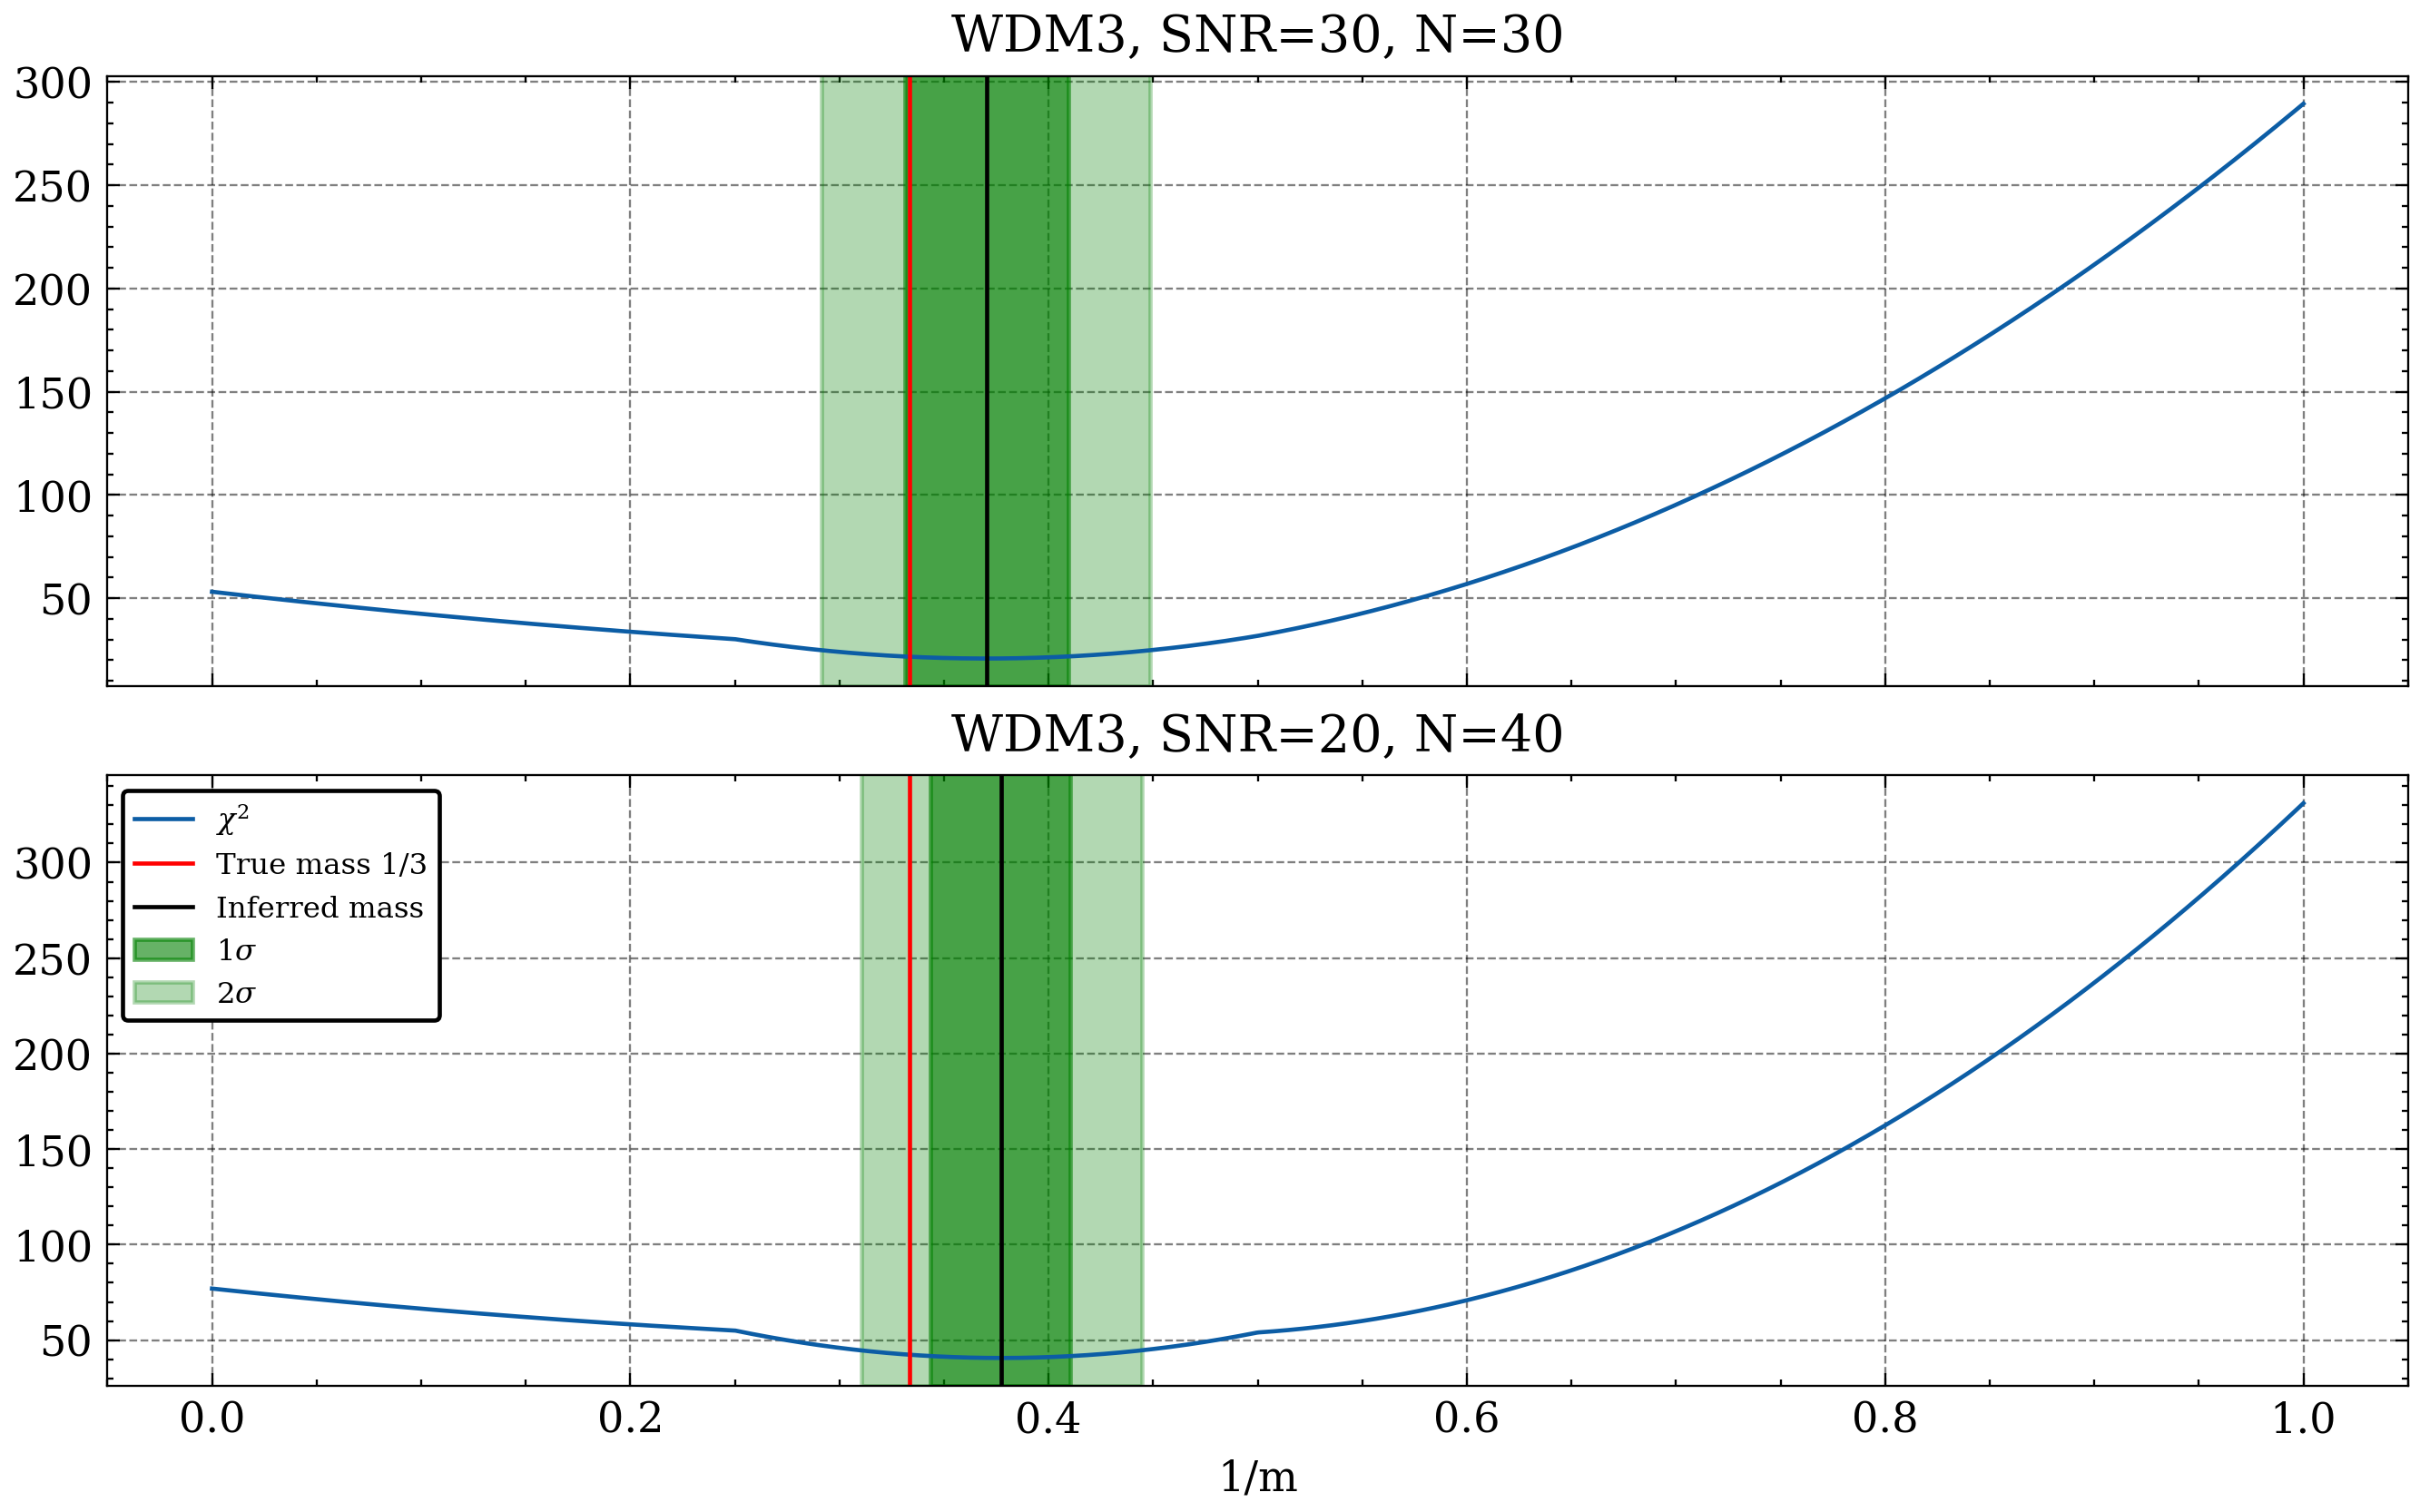
\includegraphics[width=0.8\linewidth]{img/ML/SNR_vs_N.png}
    \caption{Inference predictions on WDM3 for different combinations of SNR and number of targets N.}
    \label{fig: inference snr vs n}
\end{figure}

A common compromise in an observational program with a fixed observational time is between number of targets and exposure time per target, which determines the SNR. In Figure \ref{fig: inference snr vs n} we show how prioritising SNR or the number of targets affects to infered WDM masses on the WDM3 model. In general, we find that increasing the target number leads to slighly tighter confidence regions, while increasing the SNR leads to more accurate constraints. Most crucially, observe how the true model mass is, in both cases, recovered within $2\sigma$.

We now evaluate the constraining power of the approach developed in this work. For that purporse, we assume CDM to be the true DM model and use our fiducial neural network trained on \texttt{SHERWOOD}. We then draw 450 \texttt{SHERWOOD} skewers, corresponding to 30 observed UVES spectra, post-process them with a resolution of 6 km/s, add random Gaussian noise with $\text{SNR}=30$ and use them to run our inference pipeline from section \ref{sec: inference pipeline}. Since the fit depends on the exact draw of ``observed'' skewers, we repeat this process 100 times with a random draw each time to obtain the $2\sigma$ limit distribution.

\begin{figure}
    \centering
    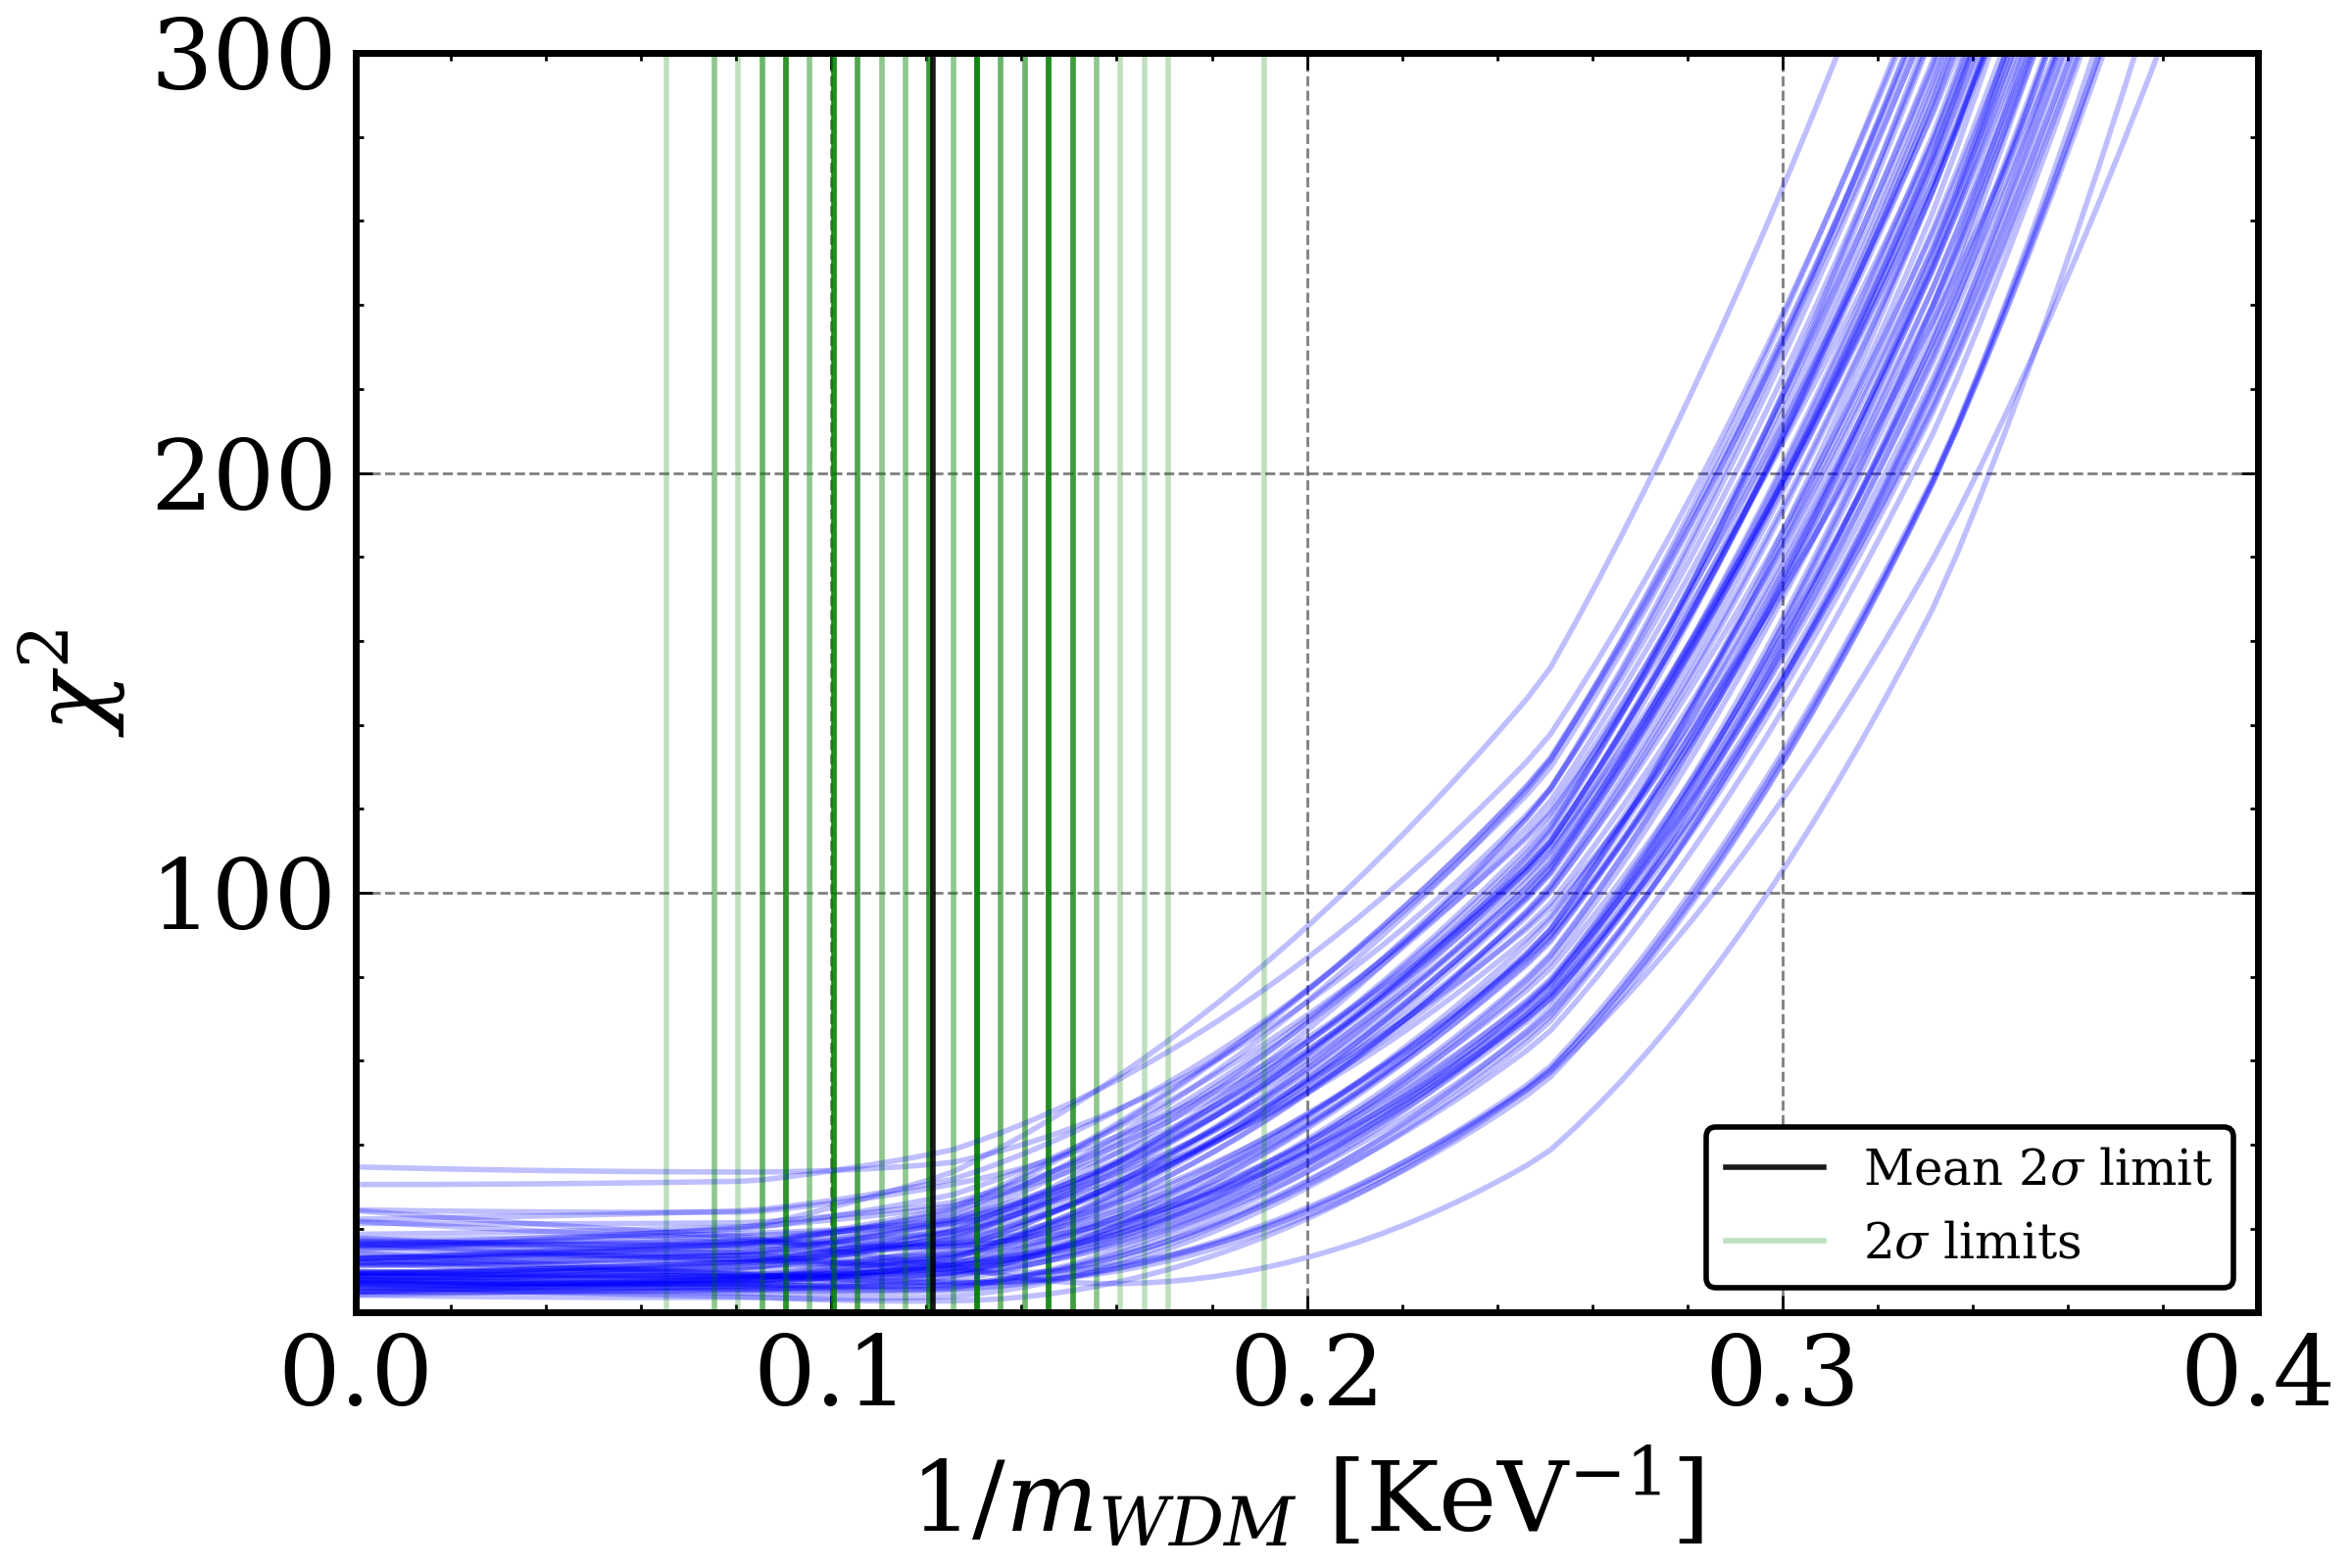
\includegraphics[width=0.8\linewidth]{img/ML/inference_cdm_sherwood.png}
    \caption{The figure shows 100 different $\chi^2$ fits on 450 \texttt{SHERWOOD} CDM skerwers and the $2\sigma$ constraints distribution as we vary the exact obsserved draw.}
    \label{fig: inference cdm sherwood}
\end{figure}
Figure \ref{fig: inference cdm sherwood} shows the distriution of $2\sigma$ limits and the mean $2\sigma$ constraint produced by this process. The mean $2\sigma$ constraint that we report for the inverse mass is $\sim 0.12$ KeV$^{-1}$, or $\sim 8.3$ KeV for the WDM model mass.

\begin{figure}
    \centering
    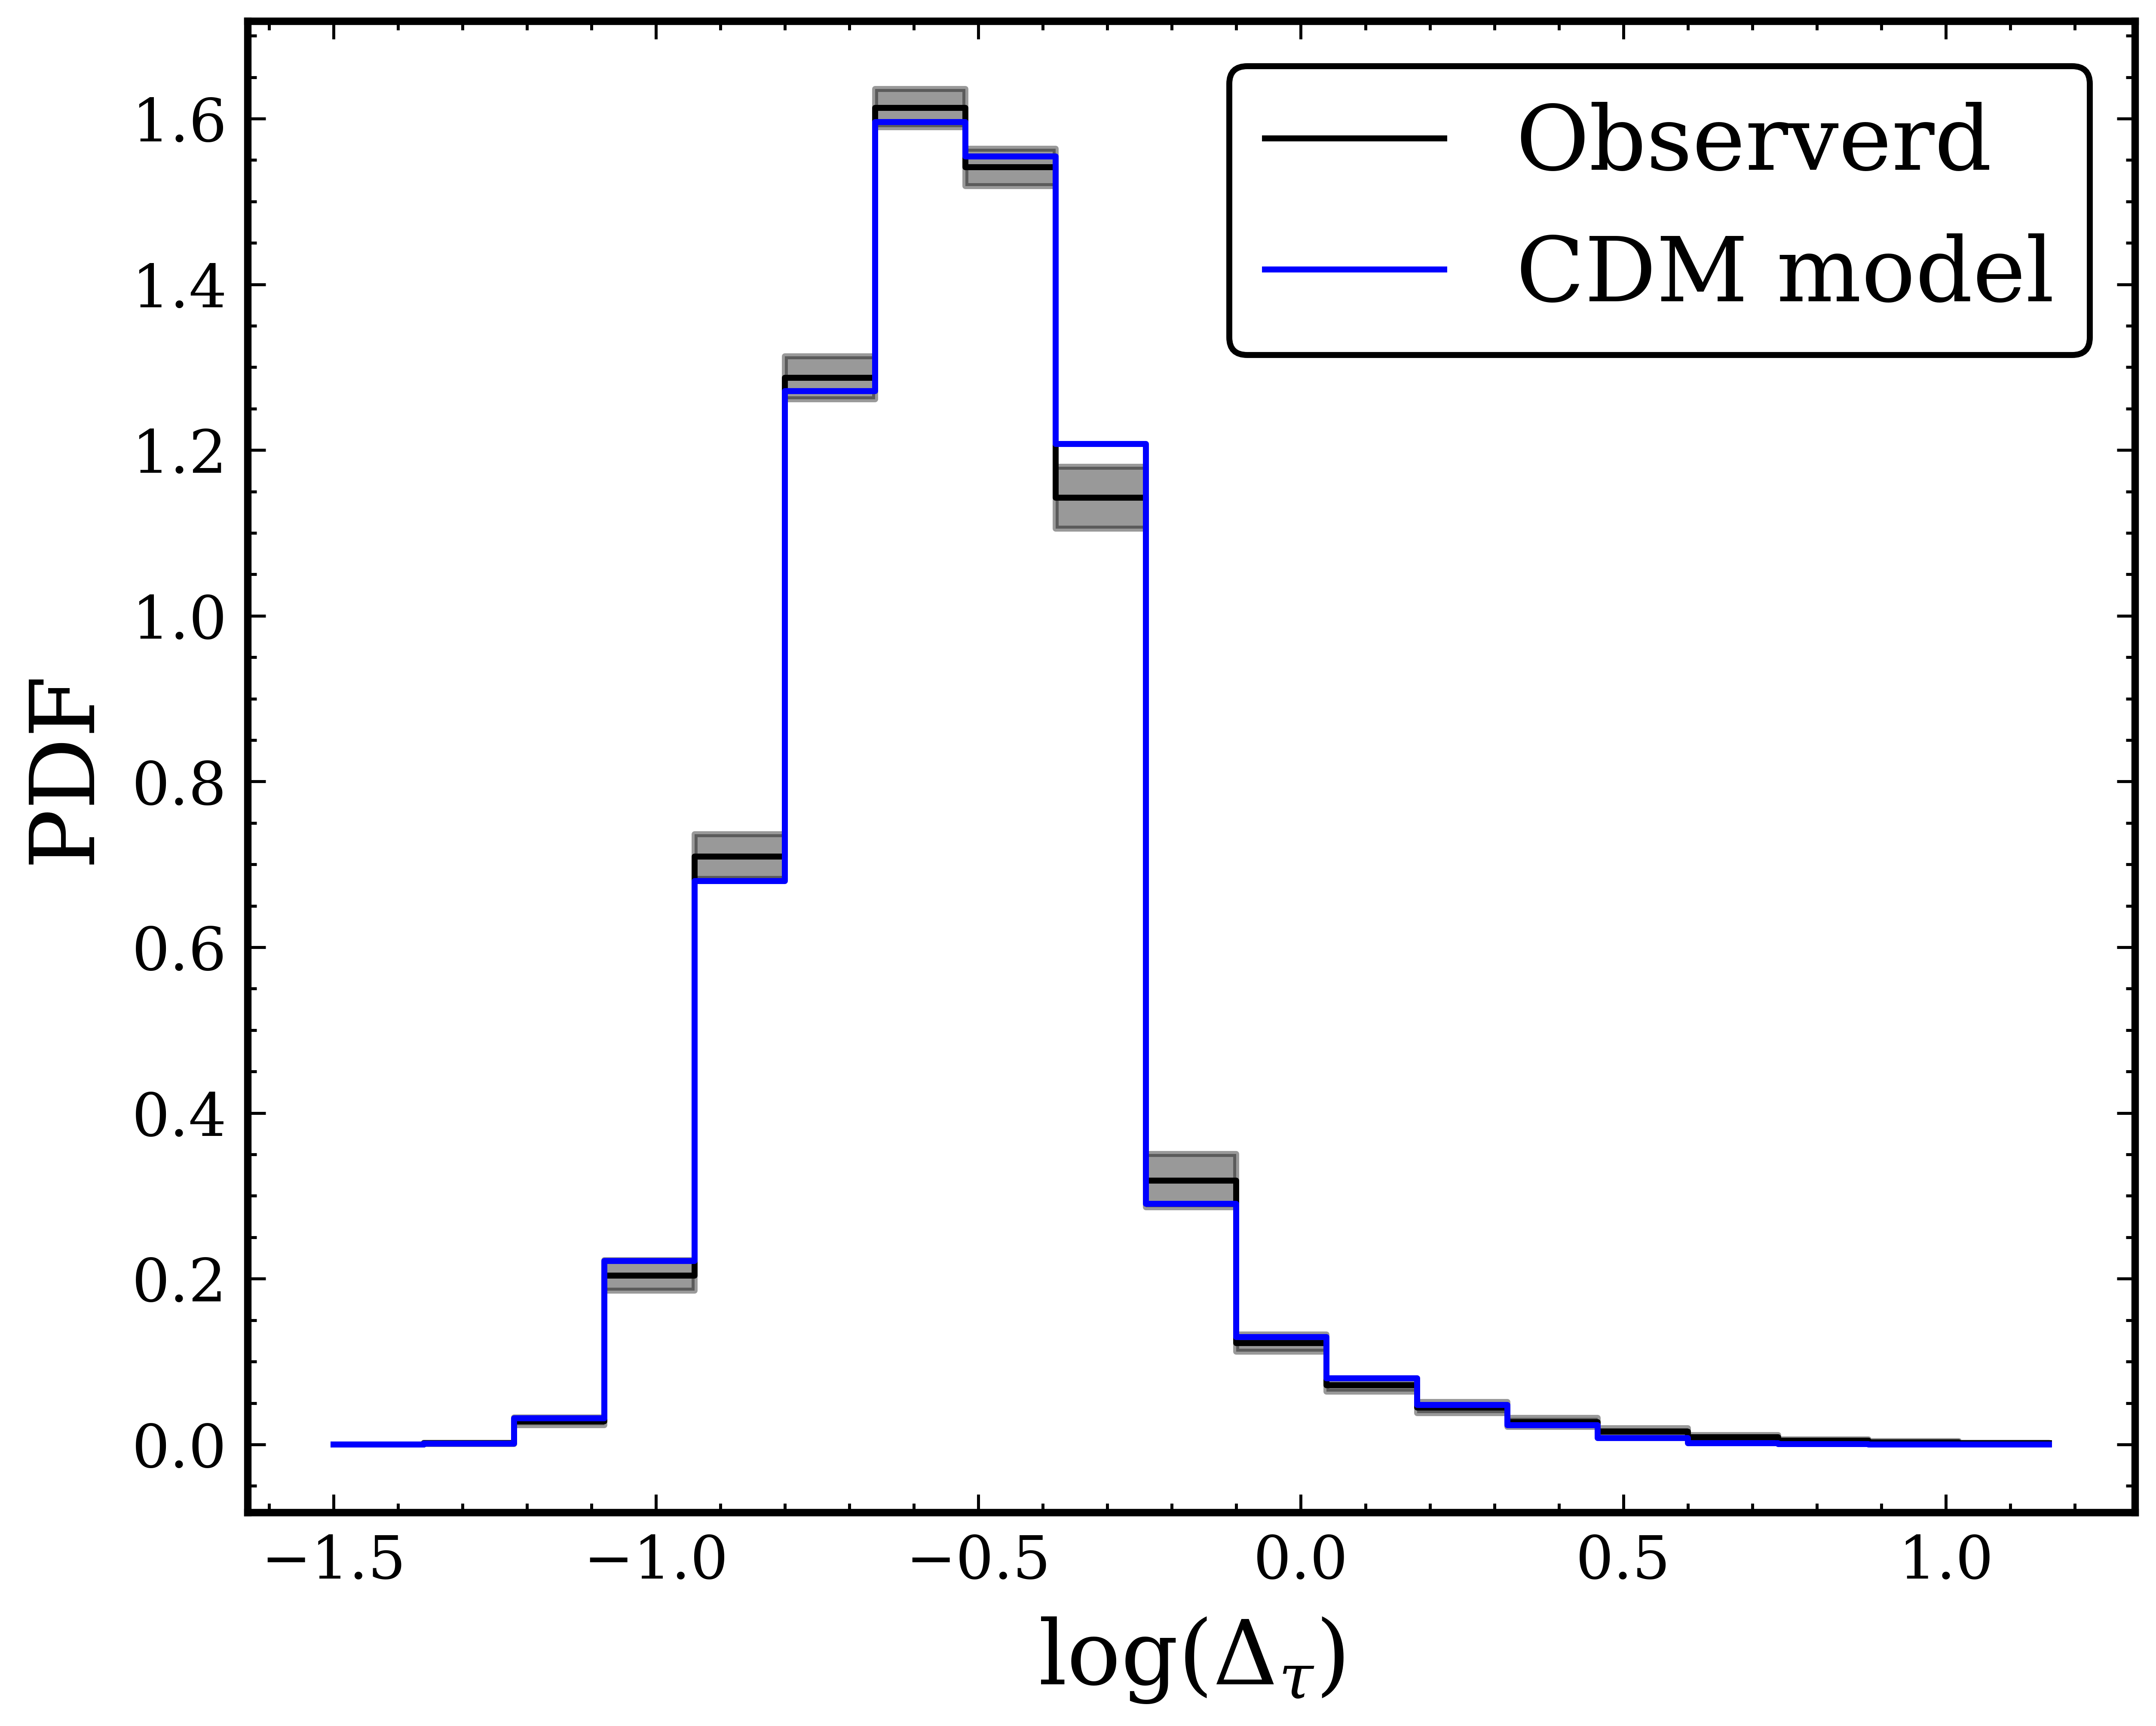
\includegraphics[width=0.6\linewidth]{img/ML/pdf_model_observed.png}
    \caption{An example observed $\Delta_\tau$ PDF recovered using 450 skewers and its uncertainties in black, plotted againt the model CDM PDF, which is the best-fit model in the $\chi^2$ test. }
    \label{fig: inference cdm PDF}
\end{figure}

To confirm that the fitting process works as expected, we plot in Figure \ref{fig: inference cdm PDF} the best fit PDF, which corresponds to the CDM model according to Figure \ref{fig: inference cdm sherwood} and an example recovered PDF from a set of 450 observed skewers. Recall that the uncertainties in the recoved PDF include the sample scatter using bootstrapping as well as the machine learning uncertainties, as we have discussed in setion \ref{sec:recovered statistics}. As expected, the observed PDF in within a $2\sigma$ distance of the model CDM PDF.

In Figure \ref{fig: wdm constraints summary} we summarise in black the current $2\sigma$ state-of-the-art constraint in the literature, using a non-ML approach. In orange, we compare the forecasted constraints from the non-machine learning approach in \cite{sherwood_wdm} to our approach in an equivalent dataset to the one used in section \ref{sec:hires test}. Compared to current limits, our forecasted constraint is a twofold improvemen, from $\sim 4$ to $\sim 8$ KeV. On the same dataset, we forecast our machine learning technique to also outperform the current pipeline in \cite{sherwood_wdm}. As a significant caveat, note that the work in \cite{sherwood_wdm} is a joint analysis not only on WDM but also on thermal parameters of the IGM, cosmological paramters, etc. The aforementioned paper encompasses a larger number of parameters with a more complex and refined approach than this work.


\begin{figure}
    \centering
    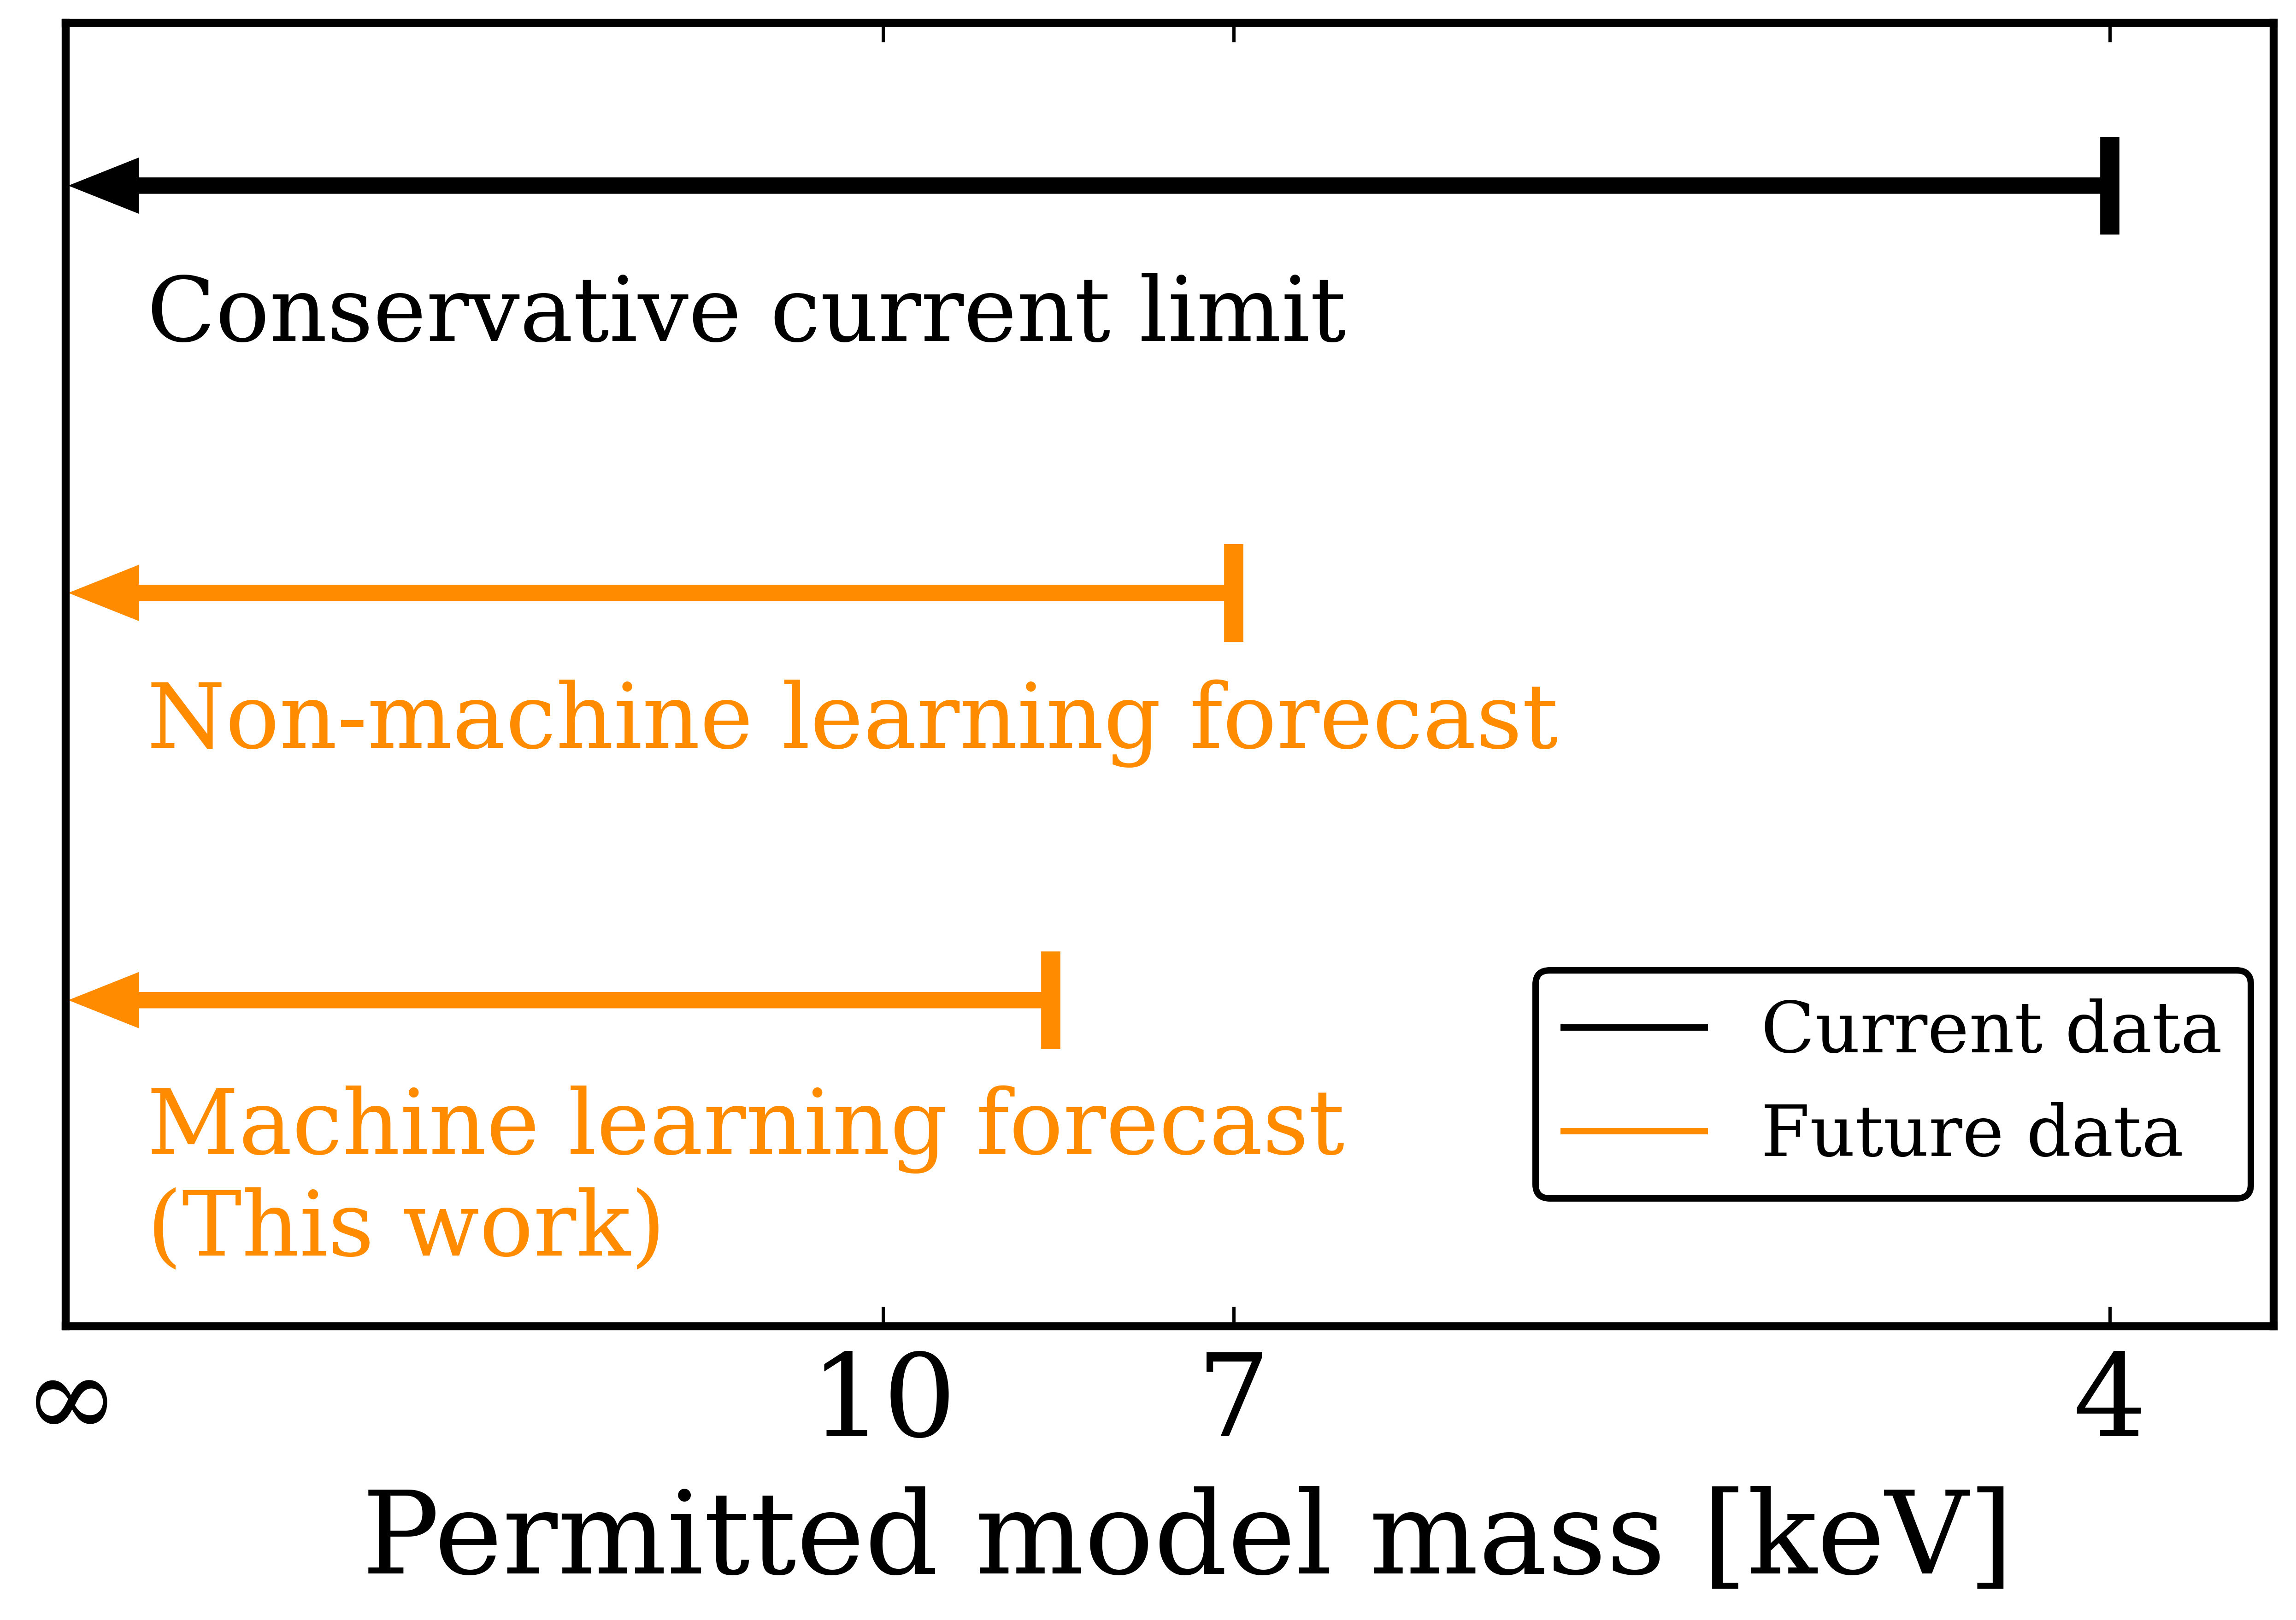
\includegraphics[width=0.6\linewidth]{img/ML/limits_summary.png}
    \caption{Summary $2\sigma$ relic WDM constraints based on \cite{sherwood_wdm} and this work.}
    \label{fig: wdm constraints summary}
\end{figure}













\section{Inference on alternative hydrodynamical codes}
In this section we test our inference pipeline on Nyx, a different hydrodynamical code. We start by discribing in a broad way the differences between the Nyx run used and the Sherwood simulations, and then we use our fiducial neural network trained on the \texttt{SHERWOOD THERMAL} suite to recover the Nyx densities and obtain the corresponding constraints.


\subsection{The Nyx code}
Nyx \cite{Almgren_2013} is an N-body and gas dynamics code for large-scale cosmological simulations. Nyx uses and Adaptive Mesh refinement (AMR) in time and space based on the Eulerian formulation of hydrodynamics, as opposed to the Lagrangian formulation used in the GADGET code emplyed by the Sherwood simulations. We expect Sherwood and Nyx runs to intrinsically show these non-physical differences related to the different hydrodynamical solvers.

In the Nyx code, dark matter is modeled as discrete Lagrangian particles, allowing the code to follow their evolution under gravity effectively. The evolution of its phase space distribution $f$ is given by the collisionless Boltzmann equation

\begin{equation}
    \begin{aligned}\frac{\partial f}{\partial t}+\frac{1}{ma^2}\mathbf{p}\cdot\nabla f-m\nabla\phi\cdot\frac{\partial f}{\partial\mathbf{p}}=0\end{aligned}
\end{equation}
where $m$ and $\mathbf{p}$ are mass and momentum and $\phi$ is the gravitational potential. $a$ is the sacale factor, obtained by using a second-order Runge-Kutta solver.
Nyx solves this phase space evolution of $f$ by sampling its distribution and evolving the particles as an N-body system. The gravitational potential is obtained by solving the Poisson equation

\begin{equation}
    \nabla^2\phi(\mathbf{x},t)=\frac{4\pi G}{a}(\rho_b+\rho_{dm}-\rho_0)
\end{equation}
where $\rho_0$ is the mean density, $\rho_b$ the baryonic density and $\rho_{dm}$ the dark matter density.
Dark matter particles are gravitationally coupled to a baryonic fluid, which is treated as an inviscid ideal gas. The gas is described by a state vector $\mathbf{U}=(\rho_b,a\rho_bU,a^2\rho_bE,a^2\rho_be)$ where $U$ is the peculiar proper baryonic velocity, $e$ the internal energy, and $E$ the total energy.
The hydrodynamical equations are approximate by a Riemann solver and can be written in the form
\begin{equation}
    \frac{\partial\mathbf{U}}{\partial t}=-\nabla\cdot\mathbf{F}+S_e+S_g+S_{HC},
\end{equation}
where $F$ is the flux vector, $S_g$ the gravity source term, $S_{HC}$ the heating and cooling term, and $S_e$ the internal energy flux.

In the rest of this section, we consider 3 Nyx runs at $z=4.4$ using CDM and 20h$^{-1}$cMpc boxes. The 3 runs different in the different reionization hisory, and are labelled by the end of reionization redshifts of $z_\mathrm{re}=6,7,8$. Each skewer has 1024 pixels. In Figure \ref{fig: nyx skewer} show an example Lyman-$\alpha$ skewer for the Nyx run with $z_\mathrm{re}=6$.


\begin{figure}
    \centering
    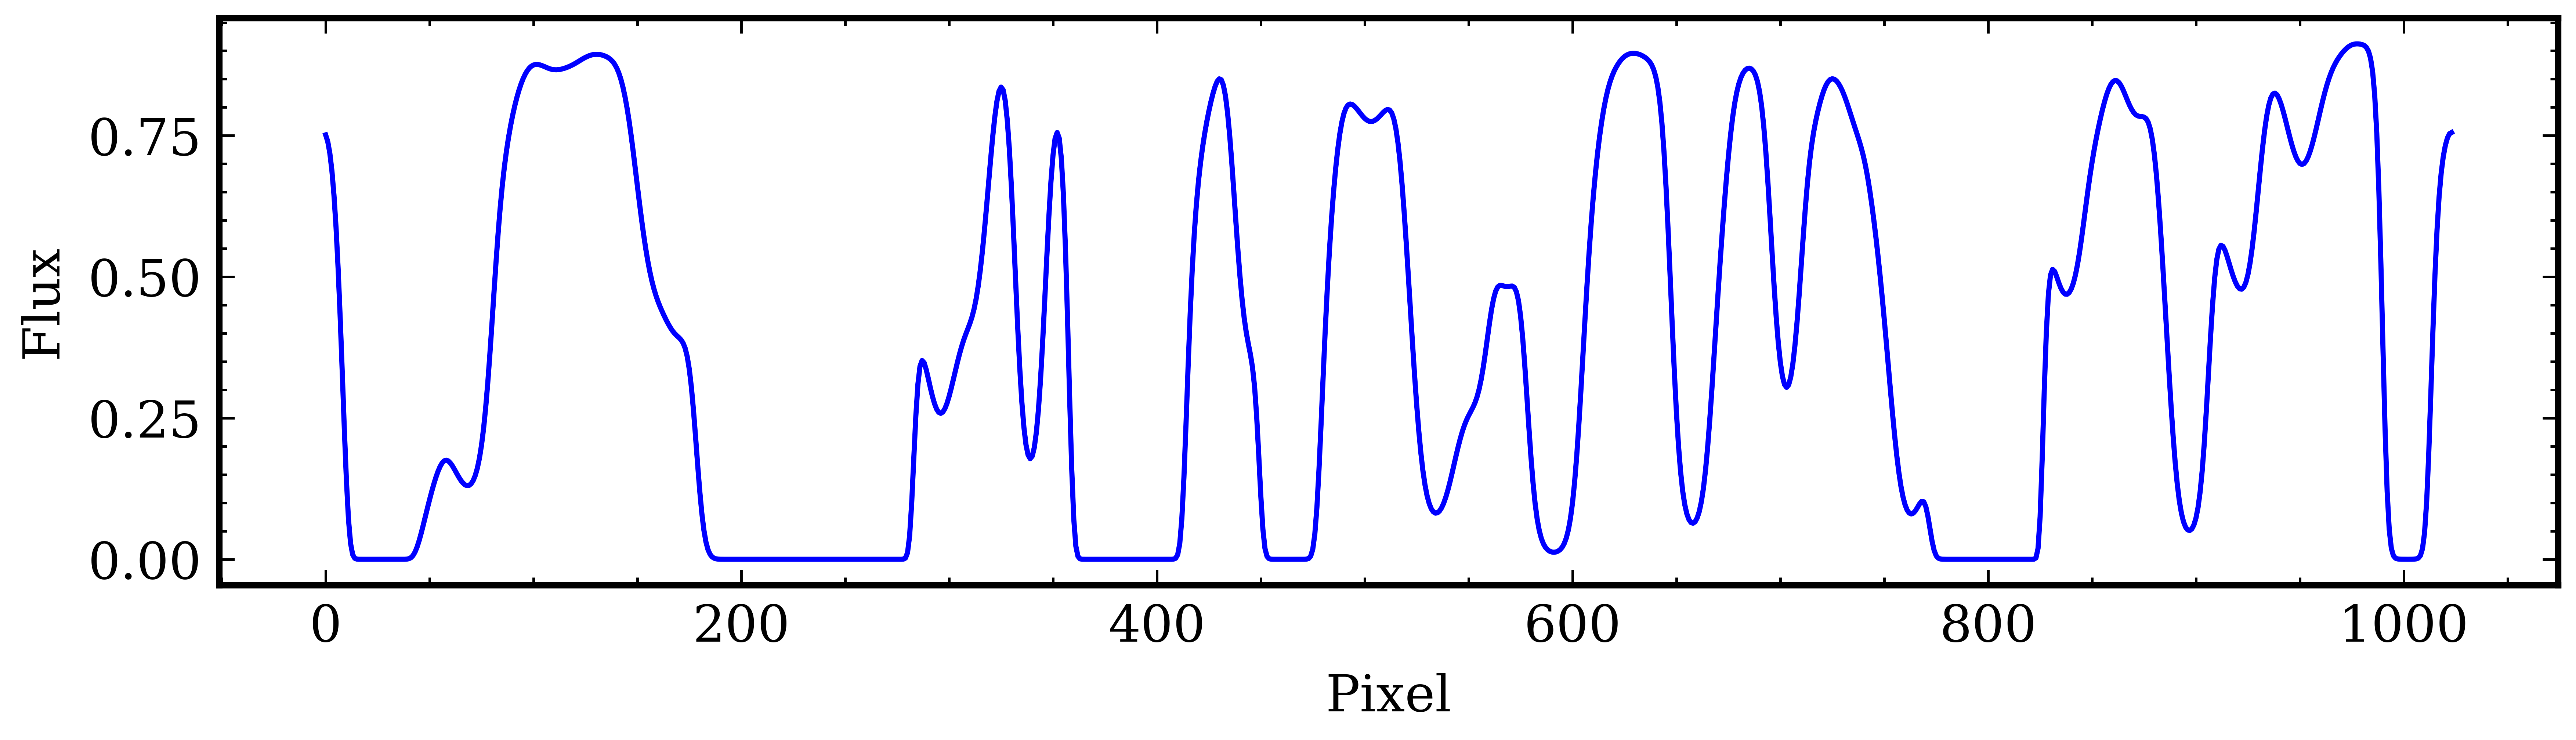
\includegraphics[width=0.8\linewidth]{img/ML/nyx_skewer.png}
    \caption{A typical Lyman-$\alpha$ skewer obtained from the Nyx runs with $z_\mathrm{re}=6$ at $z=4.4$.}
    \label{fig: nyx skewer}
\end{figure}
Since we want to test our inference pipeline, in this test we want to be as agnostic as possible about the nature of our ``observed'' Nyx spectra. If real data is observed, we would, a priori, have no information on the exact thermal history that has led to the observed field. A similar situation occurs with the Nyx runs. Our \texttt{SHERWOOD THERMAL} dataset constrains thermal models, but we have a priori no guarantee that they match the Nyx runs that we are analysing. In fact, we know that this is not the case. We visually explore the difference between the \texttt{Nyx} and \texttt{SHERWOOD THERMAL} runs, we plot the 2D distribution of pixels in the temperature-density plane. We show the result in Figure \ref{fig: nyx TD}, comparing the \texttt{Nyx} CDM run $z_\mathrm{re}=6$ to the \texttt{SHERWOOD THERMAL} CDM runs. The top panel shows the $95\%$ contours in red and black colors. The bottom ponel shows the temperature distribution at the mean density value. As can be obsered, the \text{Nyx} does not fit any of the runs in our training dataset.


\begin{figure}
    \centering
    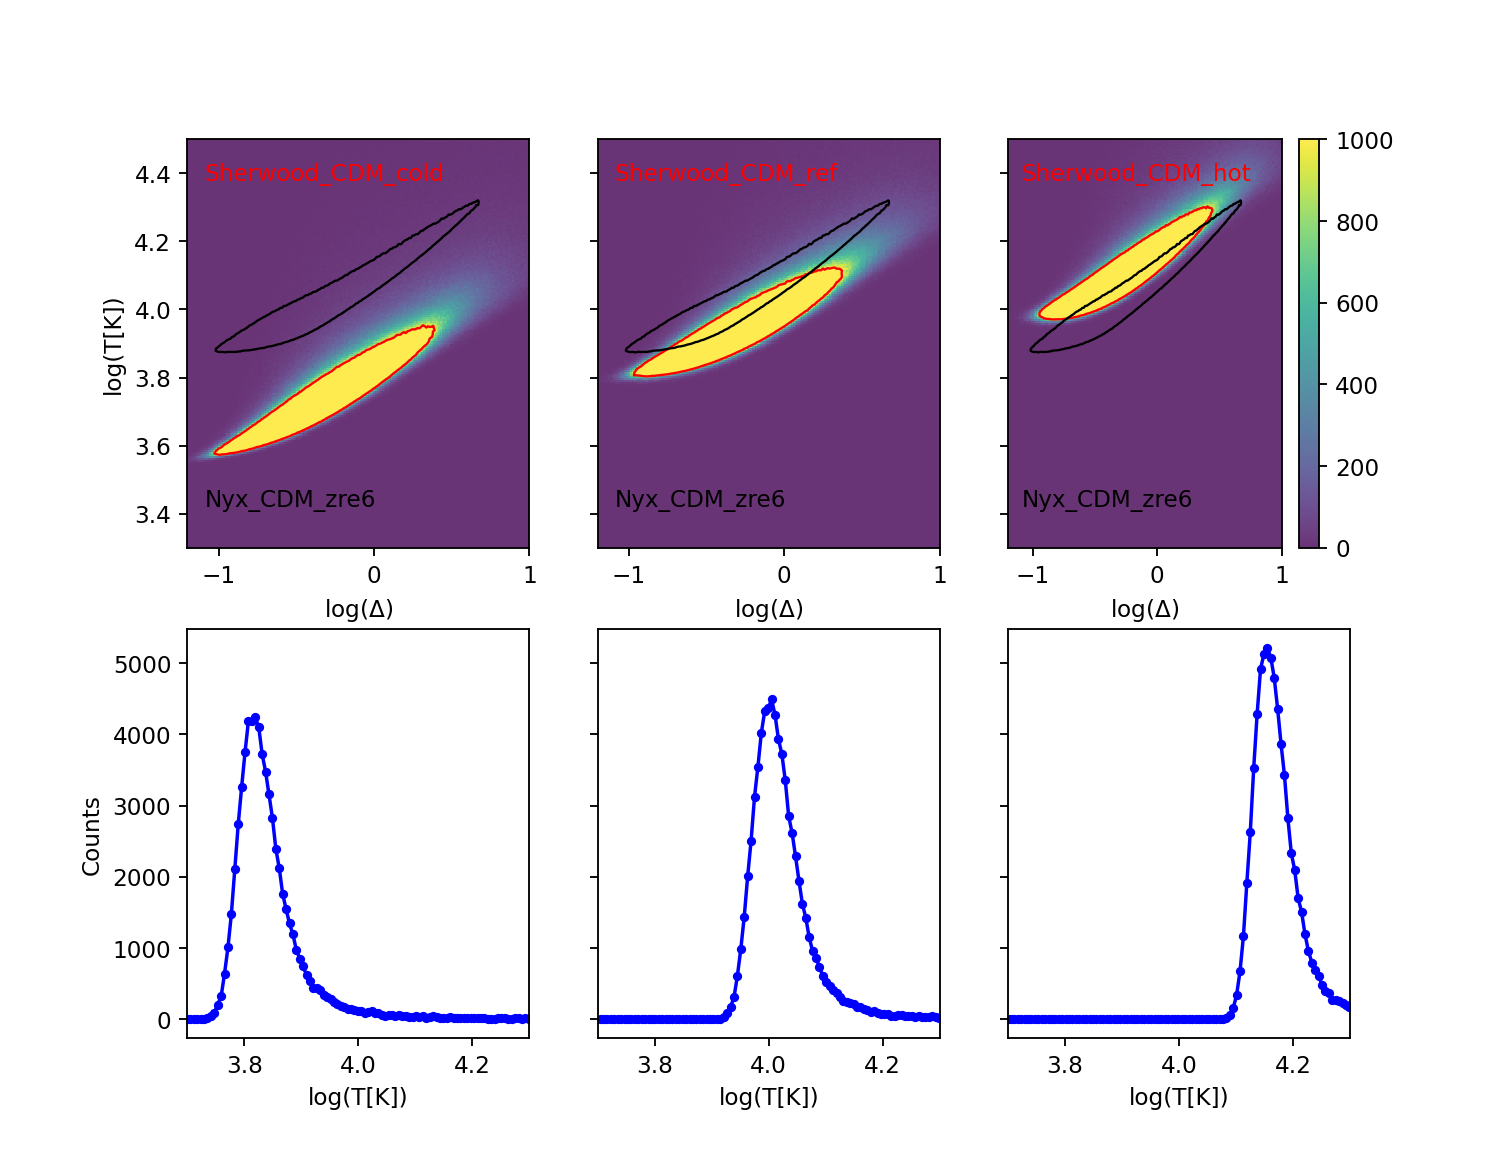
\includegraphics[width=0.99\linewidth]{img/ML/TD_plane_nyx_sher.png}
    \caption{The 2D distribution of pixels in the temperature-density plane comparing the \texttt{Nyx} CDM run $z_\mathrm{re}=6$ to the \texttt{SHERWOOD THERMAL} CDM runs. The top panel shows the $95\%$ contours in red and black colors. The bottom ponel shows the temperature distribution at the mean density value. As can be obsered, the \text{Nyx} does not fit any of the runs in our training dataset.}
    \label{fig: nyx TD}
\end{figure}

\subsection{Inference test on Nyx Lyman-alpha skewers}
We begin by evaluating the performance of our fiducial neural network with frozen weights trained on \texttt{SHERWOOD THERMAL} when predicting of skewers generated by the \texttt{Nyx} code. In Figure \ref{fig: nyx violin} we show a violin plot with the $1\sigma$ residues distribution as defined in Equation \ref{eq: residuals}. Values in the range $[0,1]$ correspond to pixels that have been succesfully recovered within a $1\sigma$ accuracy. Observer how the models with earlier reionization ($z_\mathrm{re}=7$ and $z_\mathrm{re}=8$), which have lower temperatures, have a higher recovery rate. This is likely due to the fact that our training data set contains more WDM models close to CDM, and we know that loss WDM masses and low temperate have a degenerate effect on the Lyman-$\alpha$ forest. In general, we note that the $\geq 75 \%$ of the pixels are correctly recovered. Even is the performance is slightly degraded compared to the \text{SHERWOOD THERMAL} validation, as expected, this is a strong indication that the neural network has learnt the relevant physical relations, and not potential simulation-specific correlations.

\begin{figure}
    \centering
    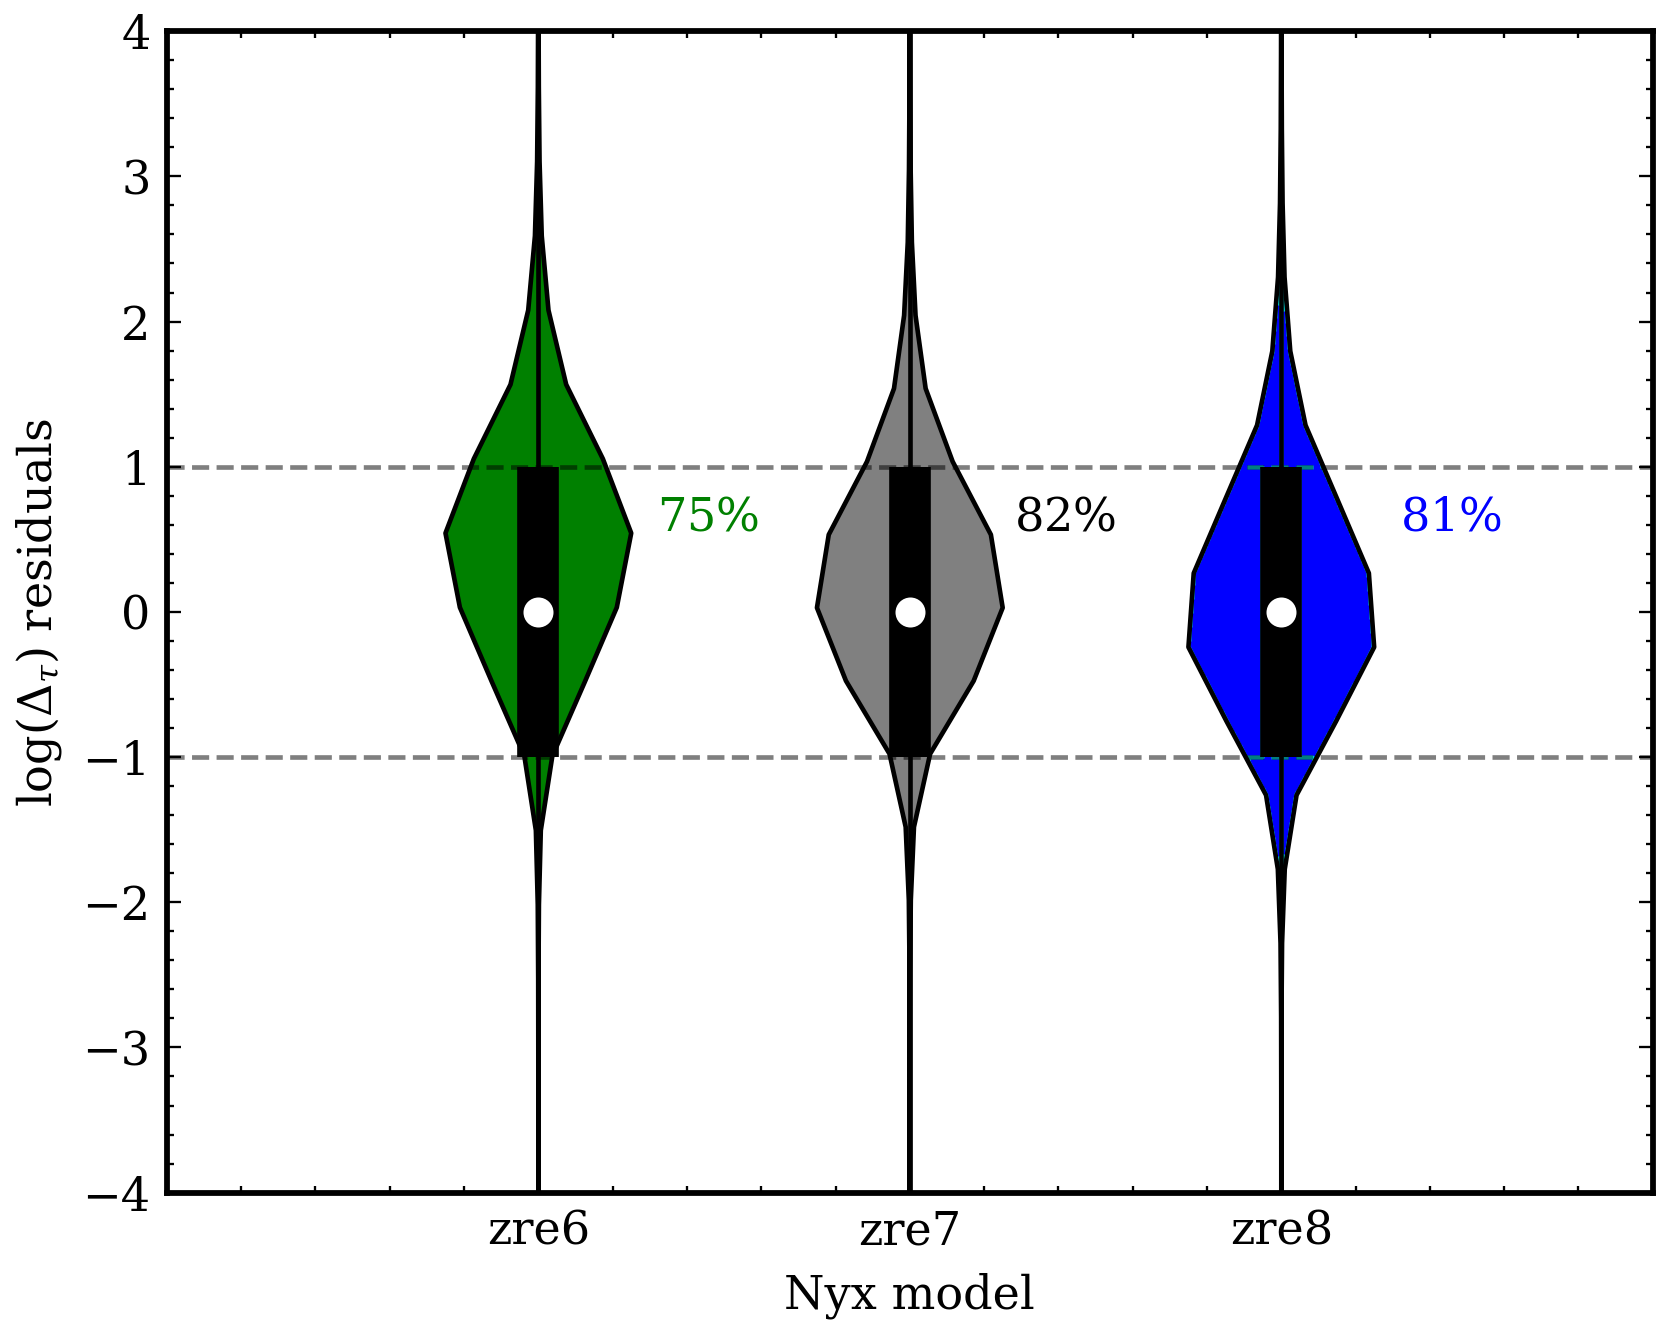
\includegraphics[width=0.8\linewidth]{img/ML/violin_nyx.png}
    \caption{iolin plot with the $1\sigma$ residues distribution as defined in Equation \ref{eq: residuals}. Values in the range $[0,1]$ correspond to pixels that have been succesfully recovered within a $1\sigma$ accuracy. Observer how the models with earlier reionization ($z_\mathrm{re}=7$ and $z_\mathrm{re}=8$), which have lower temperatures, have a higher recovery rate. This is likely due to the fact that our training data set contains more WDM models close to CDM, and we know that loss WDM masses and low temperate have a degenerate effect on the Lyman-$\alpha$ forest. In general, we note that the $\geq 75 \%$ of the pixels are correctly recovered.}
    \label{fig: nyx violin}
\end{figure}
We then run the same inference pipeline for the $z_\mathrm{re}=6$ model as we did in section \ref{sec:hires test} with a single major difference. Since we know that the \texttt{Nyx} runs do not fit any of our thermal models (and the same circumstance will occur when using real observations), we need to utilise the fiducial neural network trained on multiple thermal modes, \texttt{SHERWOOD THERMAL}. Additionally, when fitting the recovered $\Delta_\tau$ PDF to each model PDF, we will have 3 different $\chi^2$ curves for each one of the thermal models $\{\mathrm{ref}, \mathrm{hot}, \mathrm{cold} \}$. To avoid a joint optimization problem and constraining the thermal history on top of the WDM mass (which is out of the scoop of this work, and also unrealisitc since we are not using a fine thermal model grid), we will select the thermal model that minimises the $\chi^2$ value, that is
\begin{equation}\label{eq: chi thermal def}
    \mathrm{min}_{t,m} \, \, \chi^2(t,m),
\end{equation}
where $t\in \{\mathrm{ref}, \mathrm{hot}, \mathrm{cold} \}$ and $m$ labels the continously interpolatted inverse warm dark matter mass. We compute $\chi^2(t,m)$ and find that the ref and hot model produce similar $\chi^2$ values, while the cold model has $\chi^2 \sim 1000$, as expected from Figure \ref{fig: nyx TD}. Both the ref and hot models produce a similar $2\sigma$ lower bound on the WDM mass: $m_{\mathrm{WDM}} \gtrsim 10$ KeV. Compared to section \ref{sec:hires test}, the results are fairly similar, showcasing the robustness of our approach.

































\section{WDM constraints from SQUAD DR1 observational data}\label{sec:inference squad}
We begin applying our density recovery and WDM mass inference pipeline to a set of 6 observed quasar sightlines from the SQUAD DR1 survey \cite{Murphy_2018}. Since we are working with observational data, we will always train the model with the complete \texttt{SHERWOOD THERMAL} dataset that includes varied thermal histories and WDM masses. Note that since we are not trying to cosntraint the thermal history (or other parameters that can affect the Lyman-$\alpha$ forest), we should ideally use a training set that includes as much variation as possible to make sure the neural network can perform in a scenario where we ignore the true thermal history.

Our SQUAD DR1  data consists of 6 Lyman-$\alpha$ sightlines of size 20h$^{-1}$cMpc with varied SNR (see table \ref{tab: squad dr1}), observed with the Ultraviolet and Visual Echelle Spectrograph (UVES) on the European Southern Observatory’s Very Large Telescope, which has an average resolution of $\mathrm{FWHM}\approx 6$km s$^{-1}$. We consider sightlines centred at $z=4.4$ for this specific application. Since each quasar has its own noise level, we retrain the same fiducial architecture with the corresponding noise level before the prediction step.

\begin{table}
    \caption[]{List of the SQUAD DR1 sightlines used, see \cite{Murphy_2018} for the reduction details, together with their emission redshift and the average continuum SNR.     
    All sightlines are 20h$^{-1}$cMpc and centered at $z=4.4$.}
    \label{tab: squad dr1}
   $$ 
       \begin{array}{p{0.4\linewidth}cc}
          \hline
          \noalign{\smallskip}
          SQUAD DR1 name &  z_{\mathrm{em.}} & \mathrm{SNR} \\ 
          \noalign{\smallskip}
          \hline
          \noalign{\smallskip}
          J004054 &4.976  & 33    \\
          J021043           &4.65   &25\\
          J025019     &4.77   &     12      \\
          J030722     &4.728        &   50          \\
          J033829 &  5.032             &  14         \\
          J145147  & 4.763                 &  100         \\
          \noalign{\smallskip}
          \hline
       \end{array}
   $$ 
 \end{table}


We are then set to predict the recovered density fields for easch sightline. Figure \ref{fig: squad pred} shows all our SQUAD DR1 skewers togethet with the recoved $\Delta_\tau$ field.

\begin{figure}
    \centering
    \includegraphics[width=0.7\linewidth]{img/ML/SQUAD_pred.png}
    \caption{All 6 sightlines from the SQUAD DR1 sample in Table \ref{tab: squad dr1}. As can be seen, the noise levels vary, depending on the exposure time to the target. All sightlines are 20h$^{-1}$cMpc and centered at $z=4.4$. We show the recovered density field by our fiducial architecture trained on \texttt{SHERWOOD THERMAL} and retrained with the noise specifications of each target.}
    \label{fig: squad pred}
\end{figure}

We now compute the $\chi^2(t,m)$ for all 3 thermal models, which are minimised for the respective CDM run as expected, and find that the thermal model producing a minimal $\chi^2$ is the cold. In Figure \ref{fig: squad chi pdf} we show, in the left panel, all 3 $\chi^2$ curves as a function of the WDM mass. The right panel shows the recovered $\Delta_\tau$ PDF from the SQUAD DR1 sample together with the best-fit model, corresponding to the CDM cold \texttt{SHERWOOD THERMAL} model. Using the best-fit thermal model, we find a lower bound on the WDM mass of $m_{\mathrm{WDM}} \gtrsim 3.8$ KeV.


\begin{figure}
    \centering
    \begin{subfigure}[b]{0.53\textwidth}
        \centering
            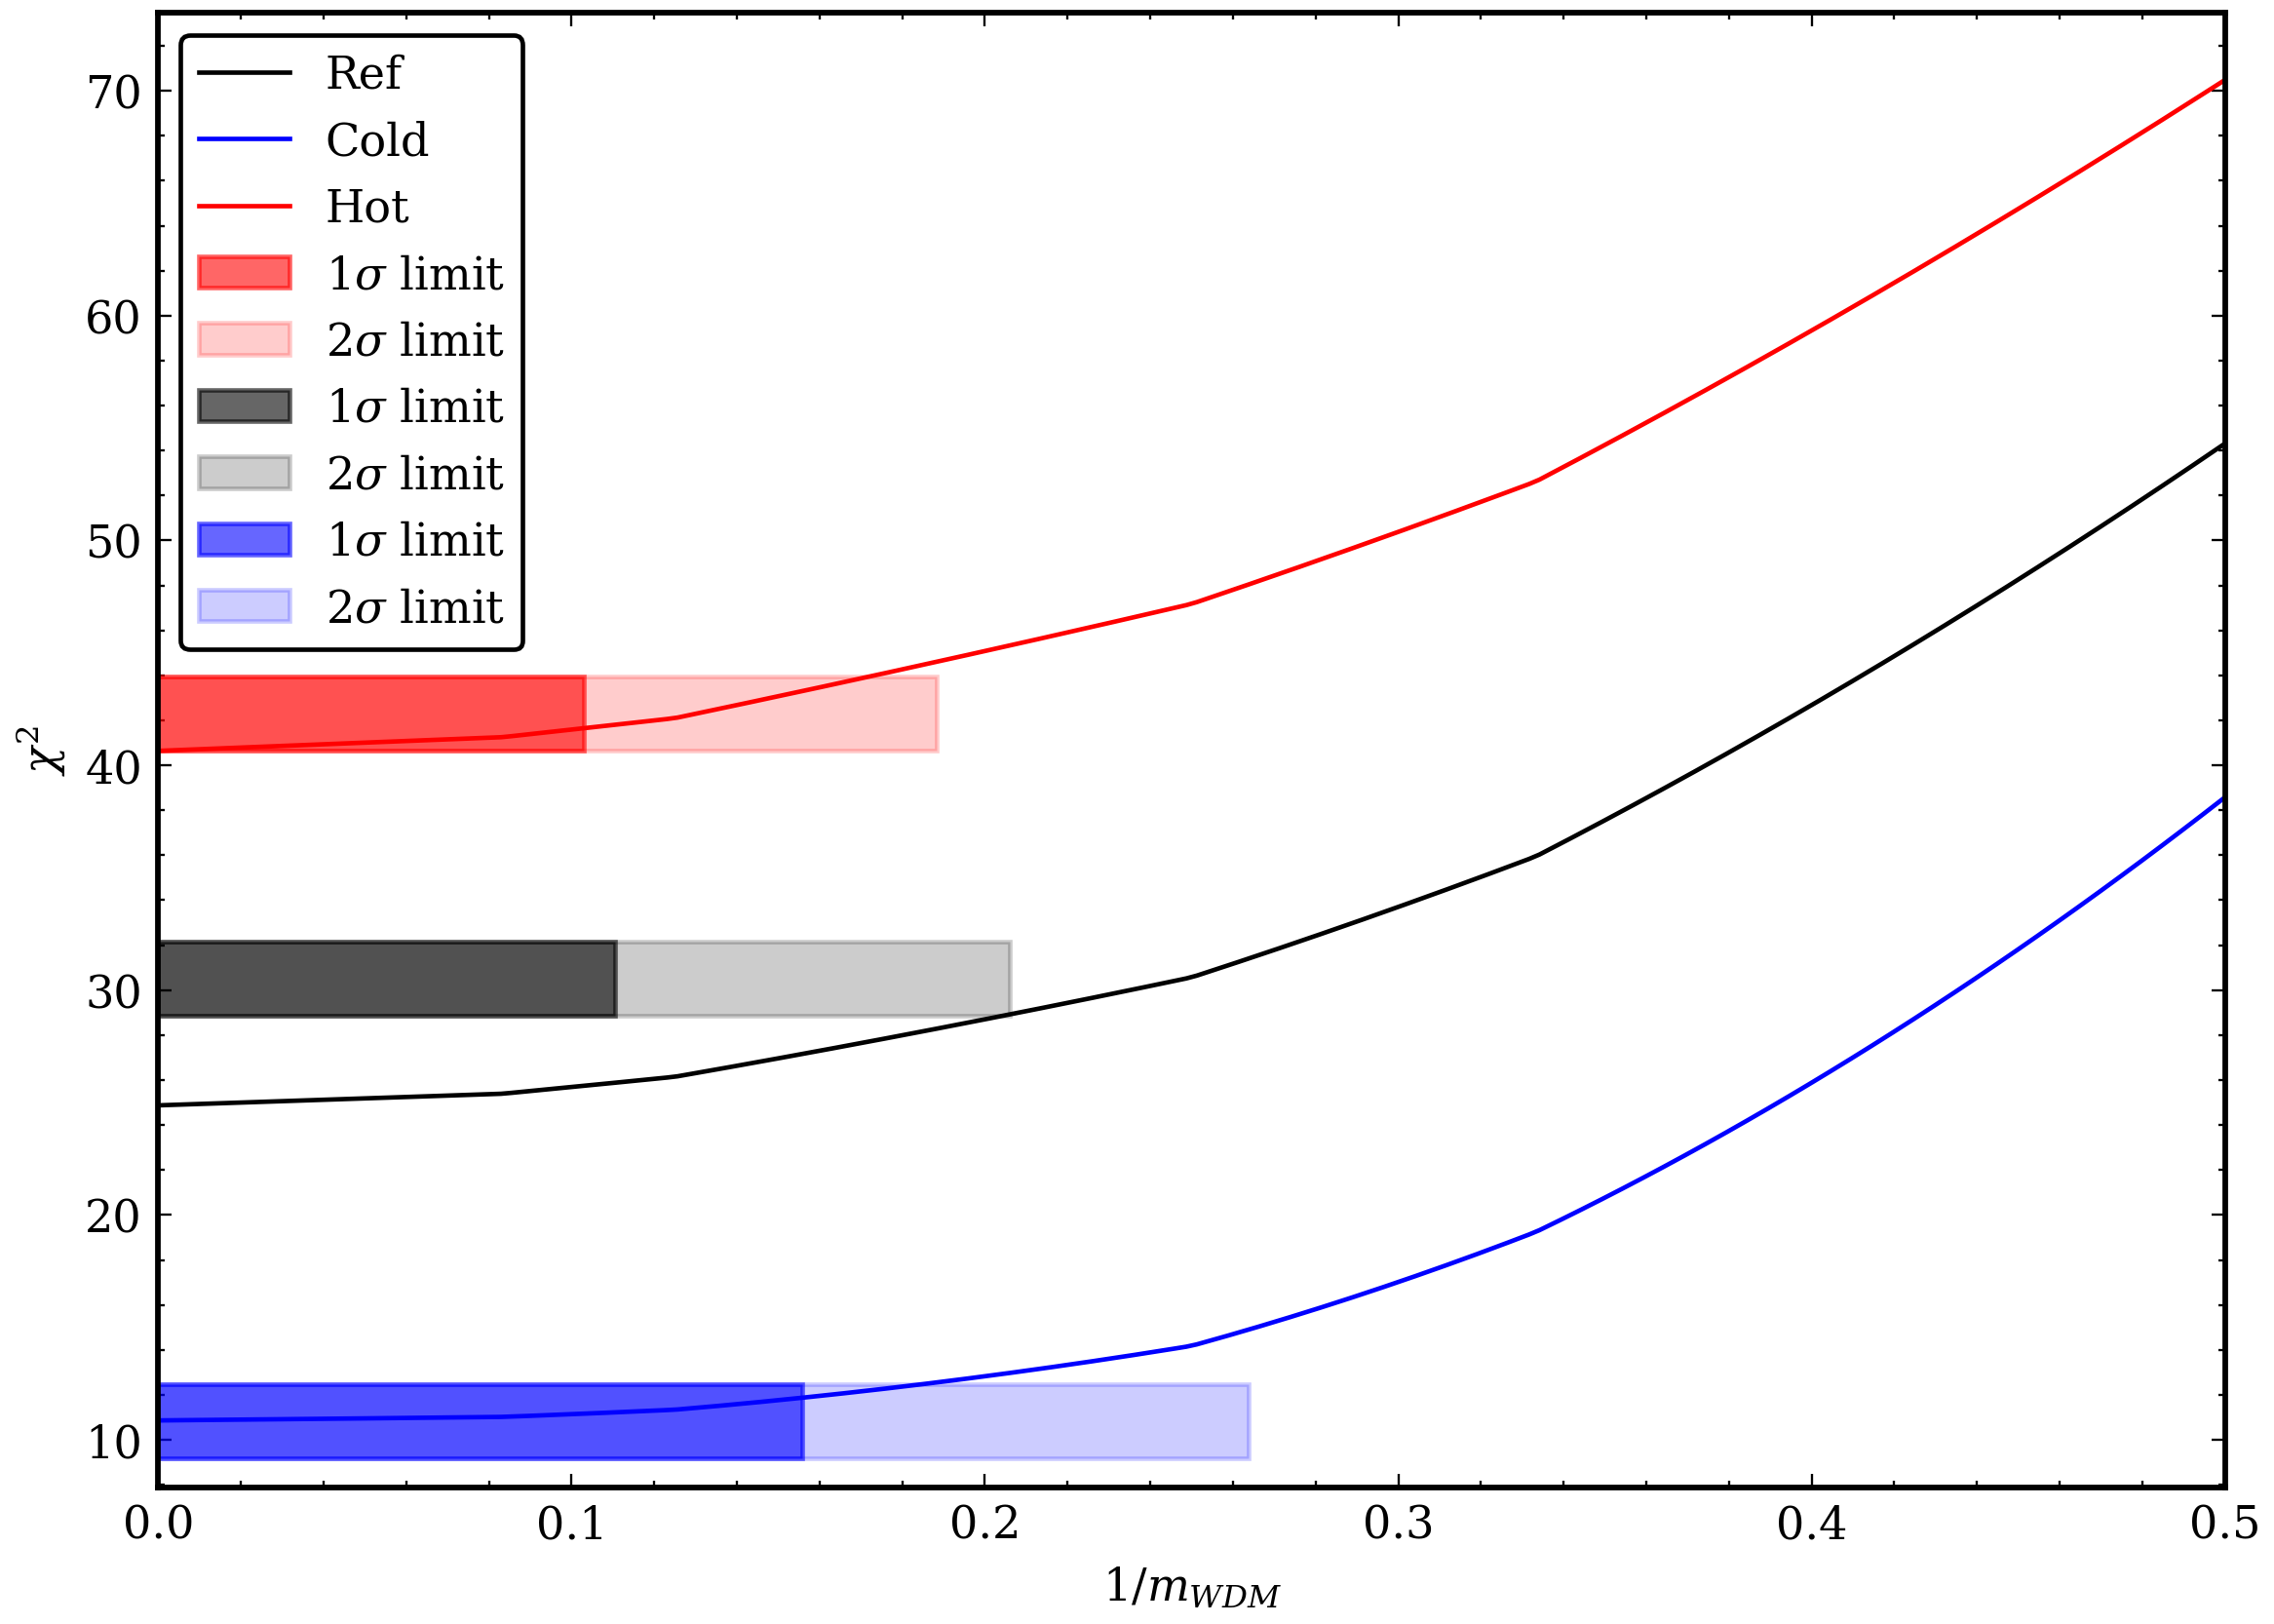
\includegraphics[width=1\textwidth]{img/ML/squad_chi.png}
    
    \end{subfigure}
    \hfill
    \begin{subfigure}[b]{0.45\textwidth}
        \centering
        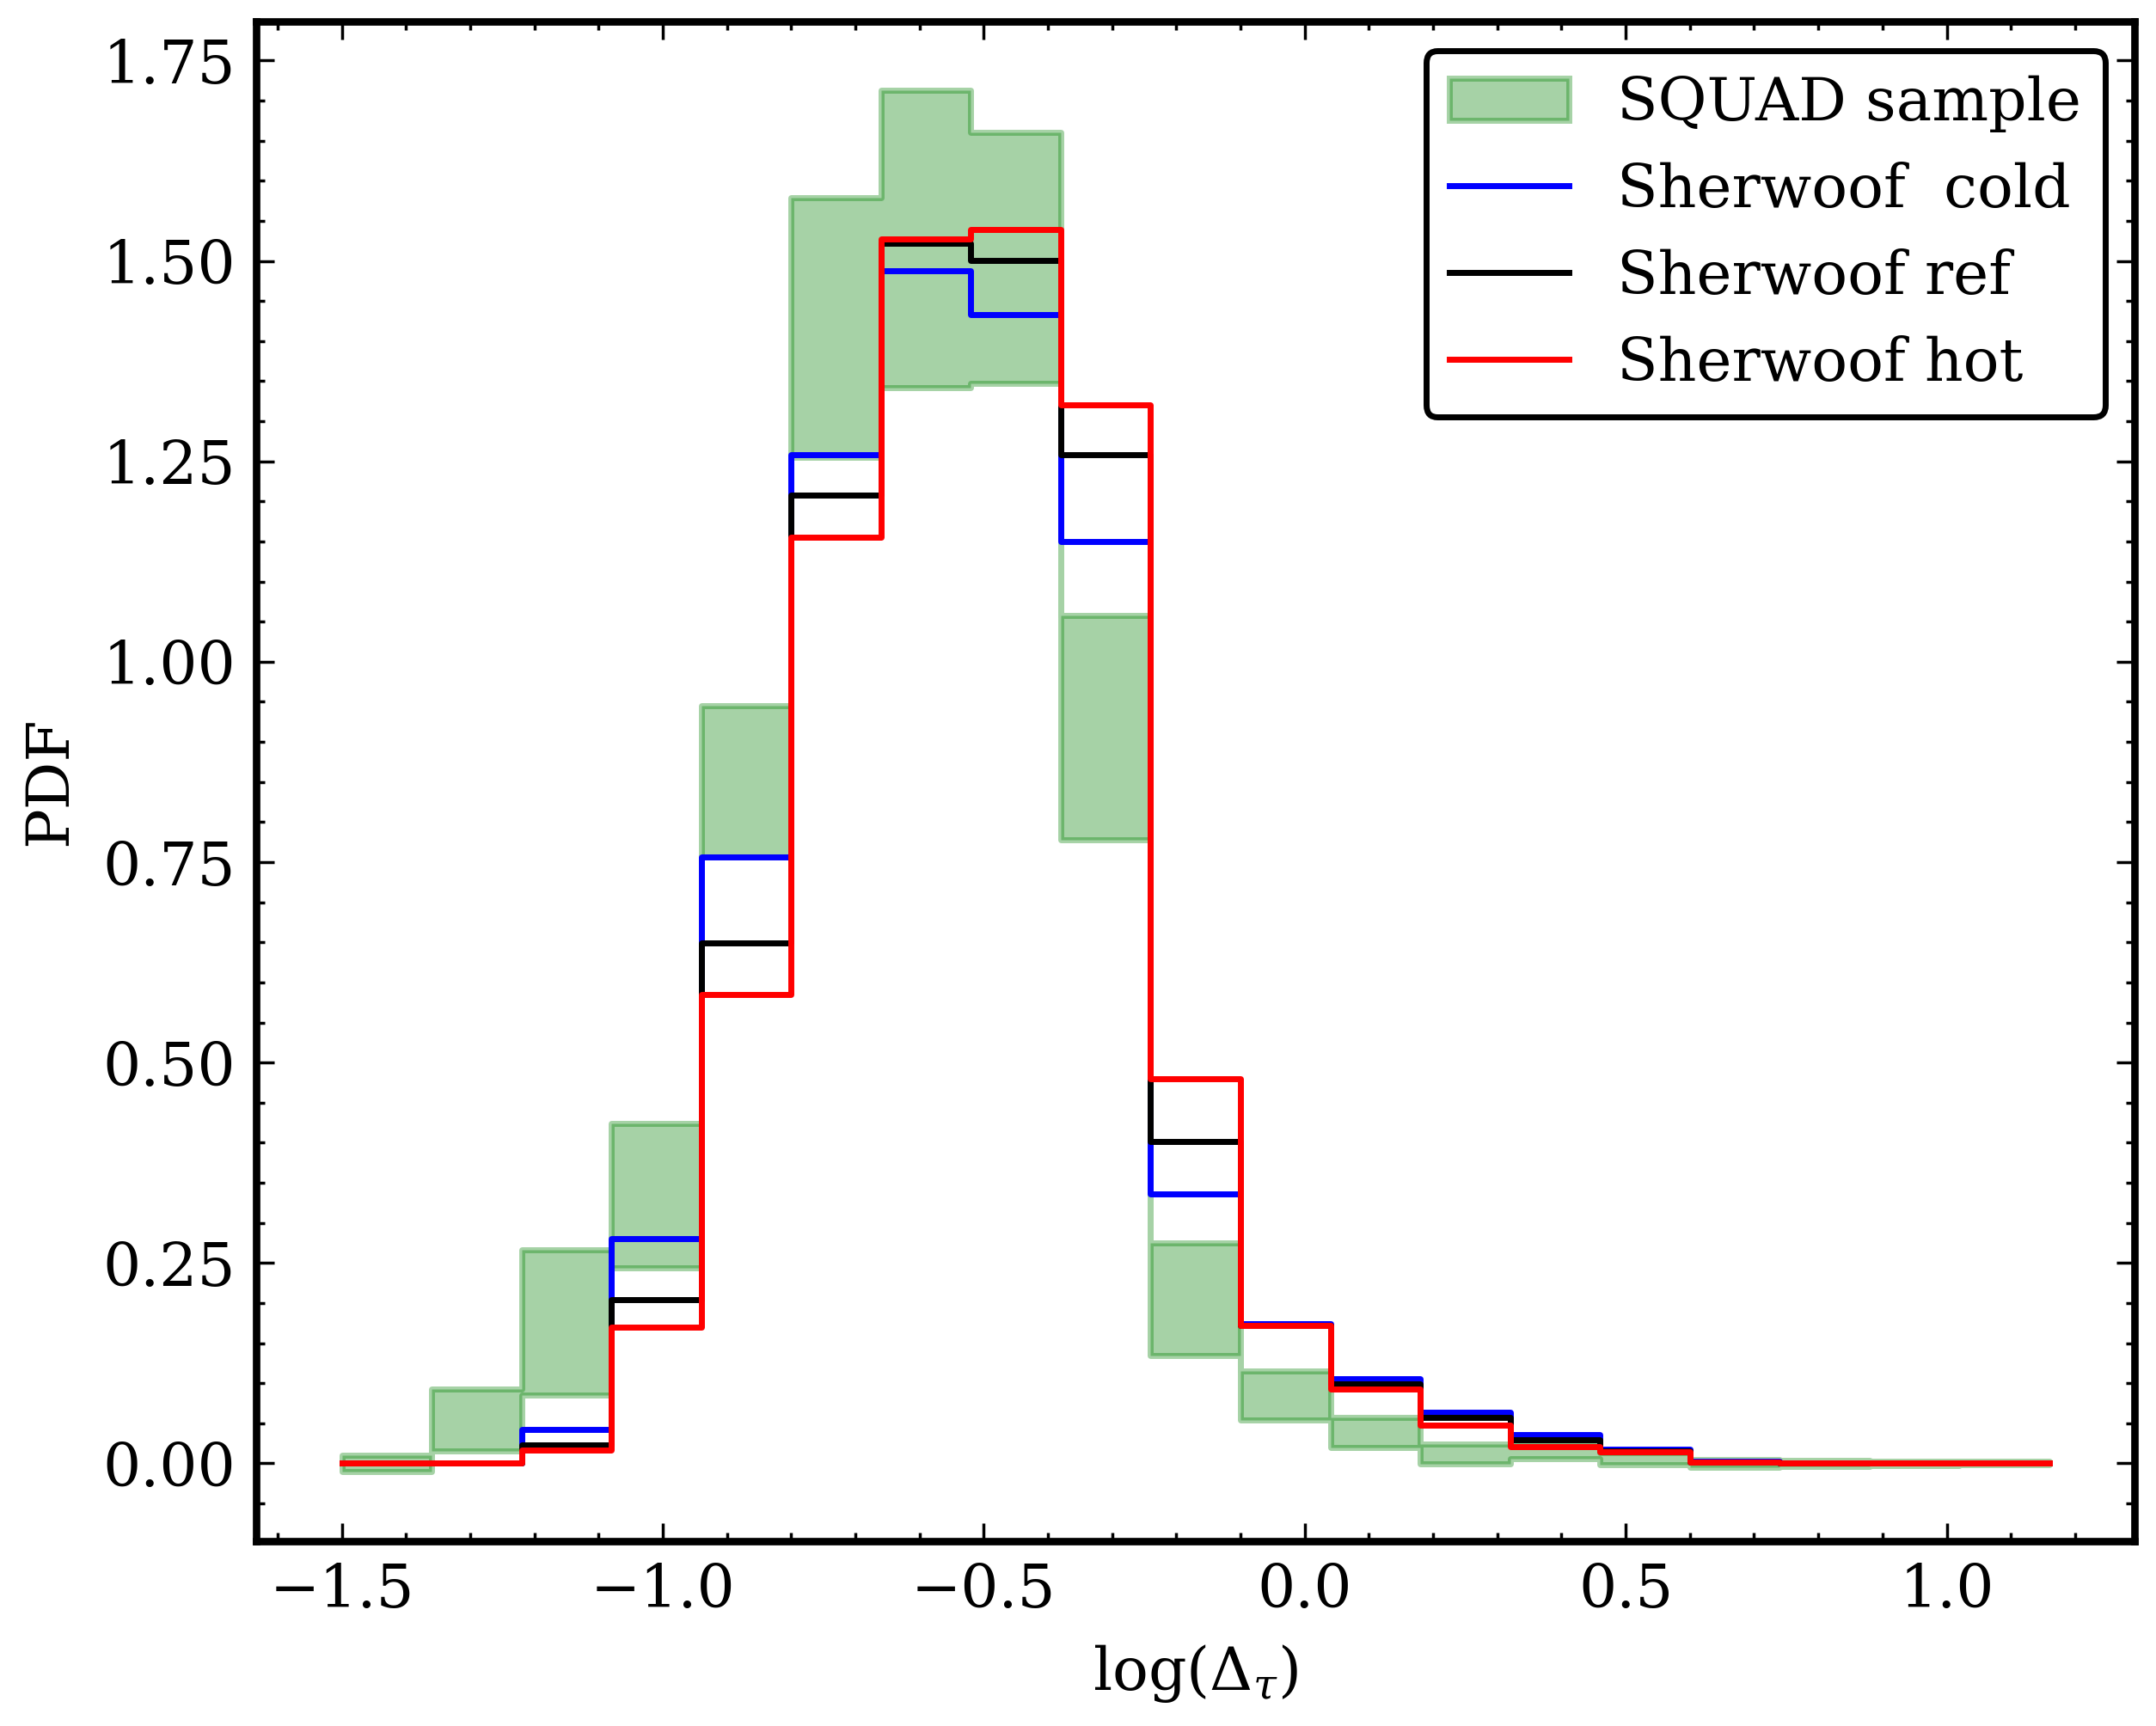
\includegraphics[width=1\textwidth]{img/ML/squad_fit_pdf.png}     
    \end{subfigure}
        \caption{In the left panel, we show all 3 $\chi^2$ curves as a function of the WDM mass, together with the $1,2\sigma$ confidence regions. The right panel shows the recovered $\Delta_\tau$ PDF from the SQUAD DR1 sample with the symmetric uncertainty envelop, together with the best-fit model, corresponding to the CDM cold \texttt{SHERWOOD THERMAL} model.
        }
        \label{fig: squad chi pdf}
\end{figure}










\section{WDM constraints from GHOST observed spectrum}\label{sec:inference ghost}
We also consider a Lyman-$\alpha$ skewer obtained from the GHOST instrument, which corresponds to the ultra-luminous quasar J0306+1853 \cite{Wang_2015} with emission redshift $z=5.363$. For this spectrum, we have a continuum reconstruction in the range $[971, 1210]$ \textup{~\AA} in the emission rest frame, with an average signal-to-noise ratio of $\mathrm{SNR}\approx 150$. We extract skewers of length 20h$^{-1}$cMpc and consider them independent in order to run the neural network predictions. In total, we obtained 13 such sightlines and discarded the range $\approx [1120,1162]$ \textup{~\AA} that contains a DLA.


\begin{figure}
    \centering
    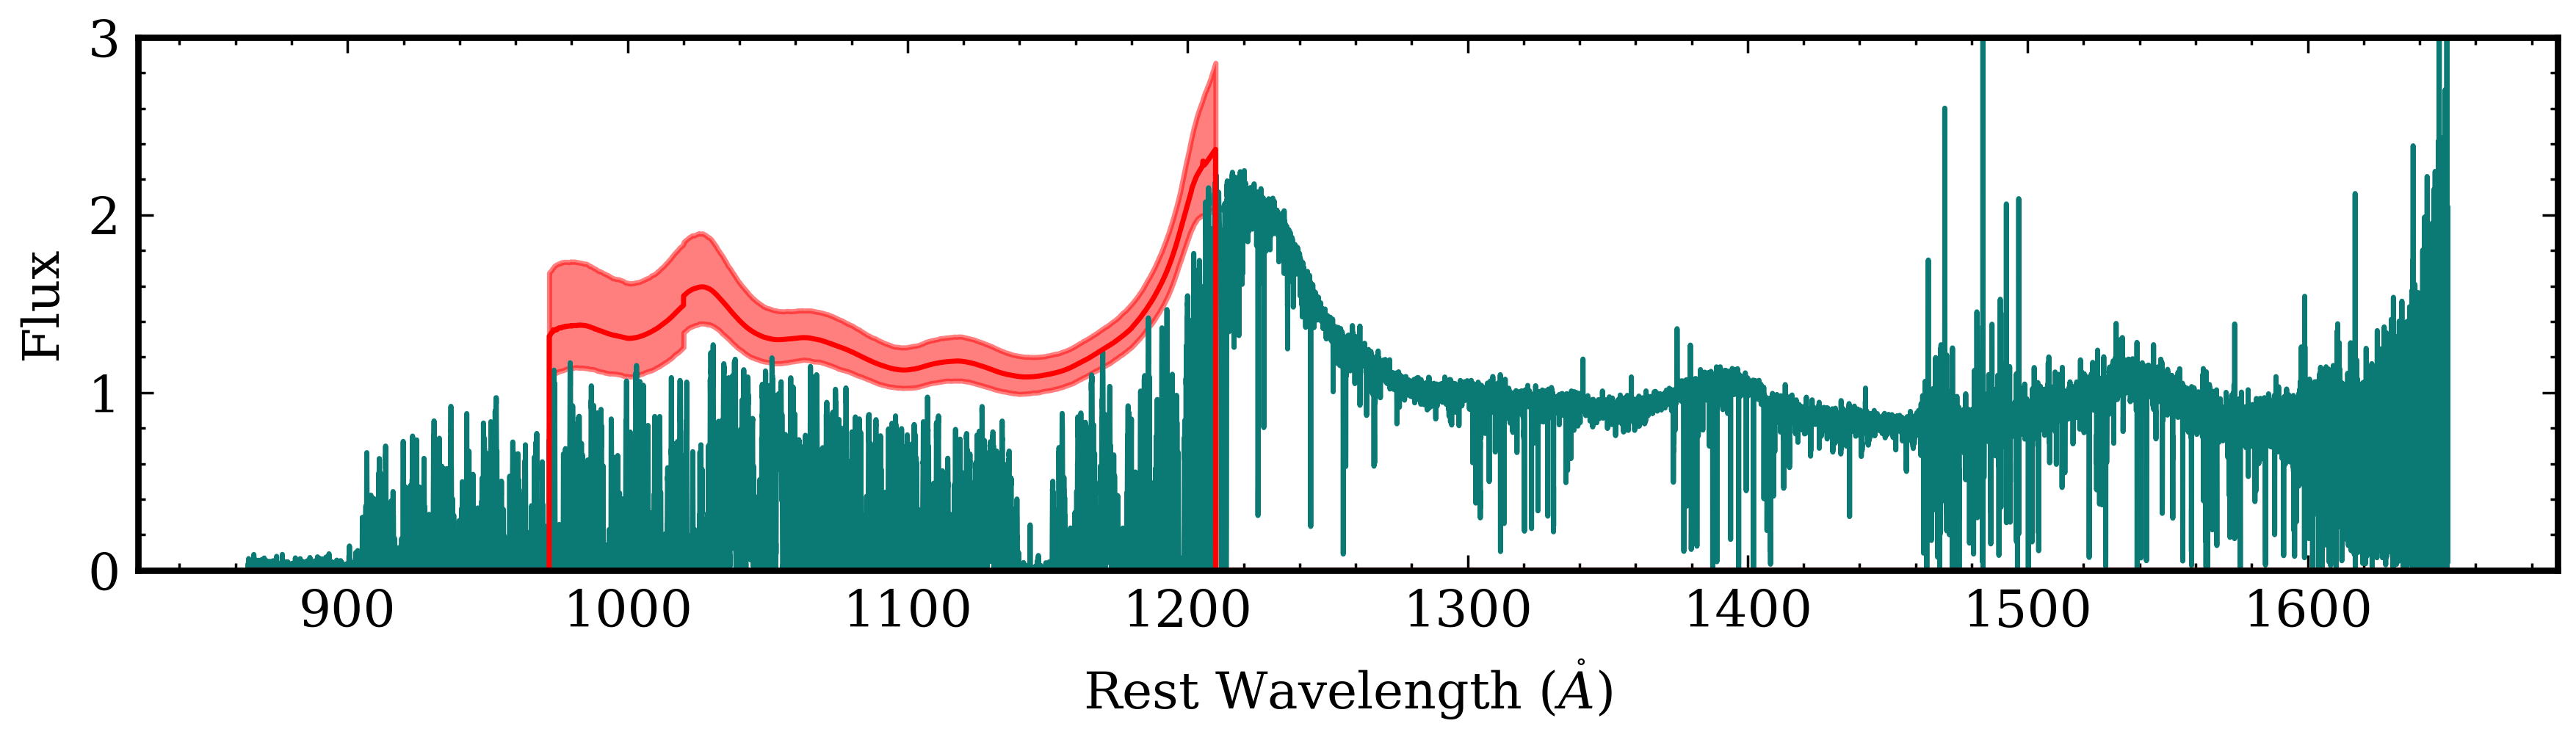
\includegraphics[width=0.7\linewidth]{img/ML/ghost_spectrum.png}
    \caption{THE GHOST spectrum for J0306+1853 \cite{Wang_2015}. The red curve shows the reconstructed continuum together with $1\sigma$ uncertainties, obtained with a PCA technique based on the spectrum to the right side of the Lyman-$\alpha$ line. Observe the DLA at $\sim 1150$ \textup{~\AA}, which we mask when analysing the Lyman-$\alpha$ forest. }
    \label{fig: ghost spectrum}
\end{figure}



Figure \ref{fig: ghost rec} shows an example 20h$^{-1}$cMpc portion of the spectrum together with the recovered density field. We split the original spectrum into 13 such skewers of the same length as the ones of the \texttt{Sherwood} dataset, and consider them independent.

We apply our WDM inference pipeline to the 13 segments of the J0306+1853 spectrum. The $\chi^2$ is minimised for the CDM model within each thermal history, and the best-fit thermal model is the \texttt{SHERWOOD THERMAL} CDM reference run. The corresponding $2\sigma$ constraint on the WDM mass is $m_{\mathrm{WDM}} \gtrsim 4.4$ KeV at $2\sigma$ confidence.




\begin{figure}[h!]
    \centering
    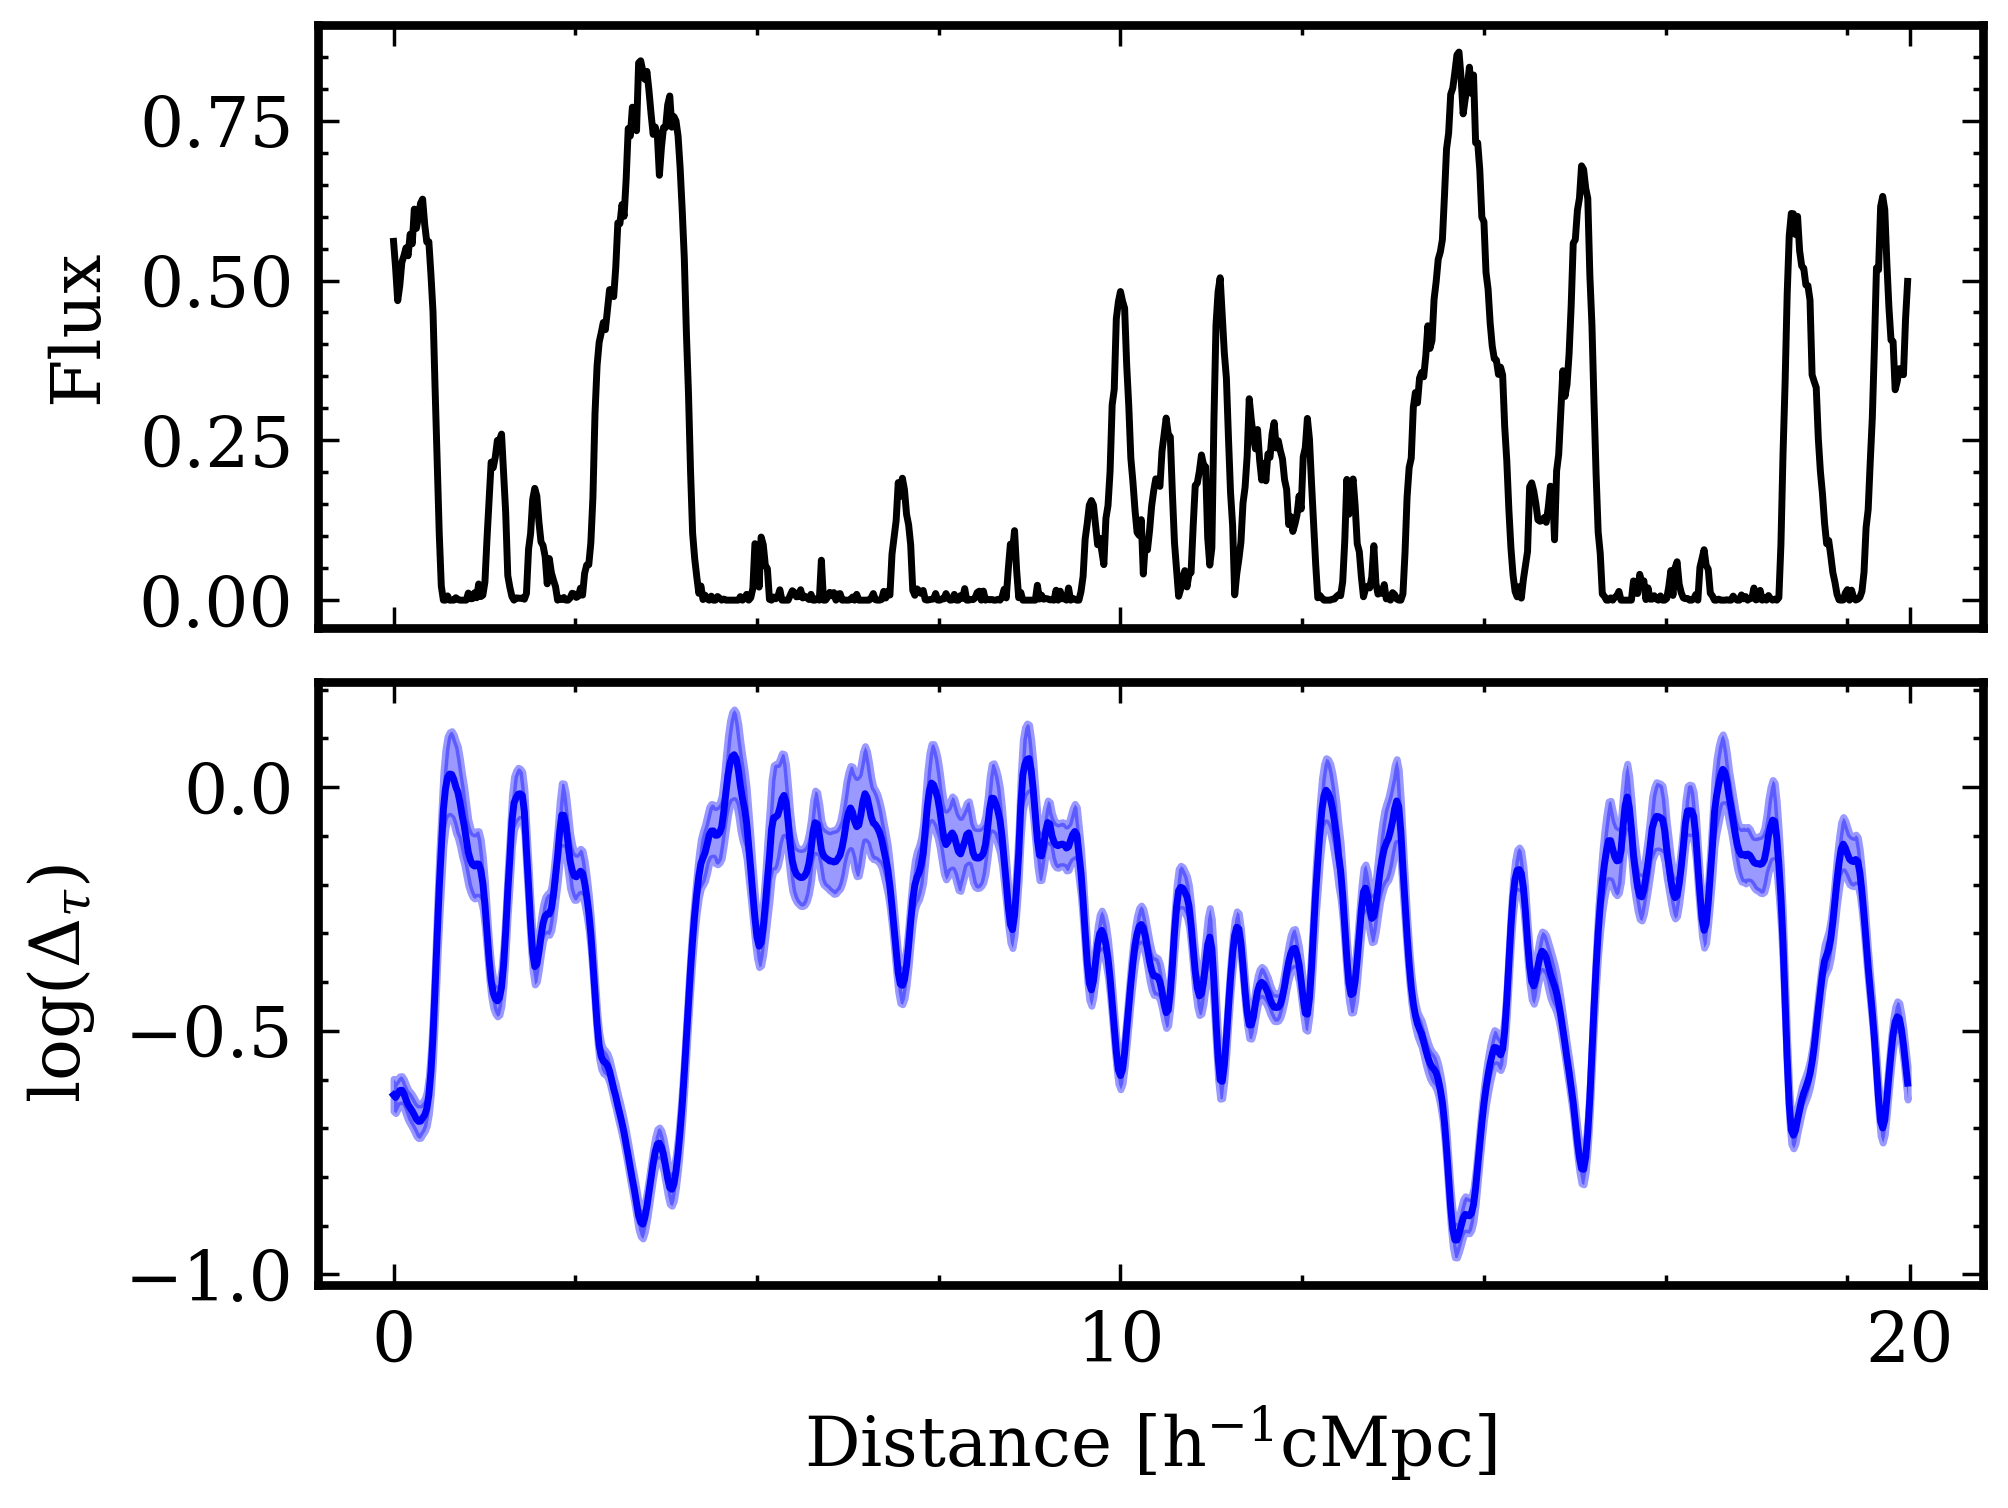
\includegraphics[width=7.5cm]{img/ML/ghost_recovered.png}
    \caption{An example 20h$^{-1}$cMpc portion of the J0306+1853 spectrum together with the recovered density field. We split the original spectrum into 13 such skewers of the same length as the ones of the \texttt{SHERWOOD THERMAL} dataset, and consider them independent.}
    \label{fig: ghost rec}
\end{figure}


In Table \ref{tab: summary constraints} we list the current state-of-the-art $2\sigma$ lower bounds on $m_{\mathrm{WDM}}$ thermal relics constraints in the literature obtained from the Lyman-$\alpha$ power spectrum. The previous efforts are based on a Bayesian inference framework to compare the observed power spectrum with the one obtained from simulated data. In contrast, in our work, we do the inference directly on the non-observable density field level. The resulting bounds produced in our work are comparable to previous efforts but with the advantage of requiring substantially less observational data. For reference, in \cite{sherwood_wdm}, the constraints are obtained from 15 spectra measured along 327h$^{-1}$cMpc,  while our GHOST data consists of 13  20h$^{-1}$cMpc skewers. The tightening of the constraint from the SQUAD DR1 sample to the GHOST sample is also expected since the latter is a larger sample with lower noise.
\begin{table}[h!]
    \caption[]{List of  current state-of-the-art $2\sigma$ lower bounds on $m_{\mathrm{WDM}}$ thermal relics constraints in the literature obtained from the Lyman-$\alpha$ power spectrum. We compare them to the results of this work, obtained doing inference directly at the density field level recovered by our Bayesian neural network. }
       \label{tab: summary constraints}
   $$ 
       \begin{array}{p{0.4\linewidth}c}
          \hline
          \noalign{\smallskip}
          Source &  2\sigma\ m_{\mathrm{WDM}} \mathrm{{\ lower \ bound\ [KeV]}}  \\ 
          \noalign{\smallskip}
          \hline
          \noalign{\smallskip}
          Ir\v{s}i\v{c} et al. (2024) \cite{sherwood_wdm} & 4.1      \\
          Villasenor et al. (2023) \cite{Villasenor_2023} & 3.1      \\
          \noalign{\smallskip}
          \hline
          \noalign{\smallskip}
          This work (SQUAD DR1 sample)  & 3.8   \\
          This work (GHOST spectrum)  & 4.4        \\

          \noalign{\smallskip}
          \hline
       \end{array}
   $$ 
 \end{table}















\section{Comparison of the inference pipeline against Information Maximising Neural Networks}


The inference pipeline presented so far in this section is based on a simple $\chi^2$ fit of the $\Delta_\tau$ recovered PDFs from our fiducial NN model. This pipeline rellies on a series of contingent choices, most notably the use of the density PDFs as the summary statistics of the fields. In this section, we explore, in an agnostic way, the possiblity of using other summaries different from the $\Delta_\tau$ PDFs to perform the inference (note that other summaries such as the density power spectrum, curvature,... could potentially be used). More concretely, we will introduce Information Maximising Neural Networks (IMNNs) and use them to perform the inference within a Bayesian framework. We then compare the results of this procedure with the inerence pipeline discussed in section \ref{sec: inference pipeline}.

\subsection{Information Maximising Neural Networks}
Information Maximising Neural Networks aim at obtaining optimal summaries of data \cite{Charnock_2018}. Neural networks are used to parametrise these summaries in an agnostic way by maximising the information of the summaries with respect to the model parameters of interest.

Consider a data-generating procedure depending on some model parameters $\theta$, generating data realization $d_i(\theta)$ where $i$ labels a realization or initial seed of the simulation. We want to obtain a function $f \colon d \mapsto x$ that maps each simulation to a summary vector of the same size as $\theta$. This is, essentially, a compression algorithm. IMNNs work by transforming the original likelihood of the data, which is a priori not known, into the gaussian form

\begin{equation}
    -2\ln\mathcal{L}\left(x|\theta\right)=\left(x-\mu\left(\theta\right)\right)^TC^{-1}\left(x-\mu\left(\theta\right)\right),
\end{equation}

where $C$ is the covariance matrix of the calculated summaries with a set of $n_s$ simulations, and $\mu$ the summary mean depending on the model parameters. The information of the observed summaries with respect to $\theta$ is then the Fisher information matrix \cite{ly2017tutorialfisherinformation}:

\begin{equation}\label{eq:Fisher information}
    F_{\alpha \beta} =-\operatorname{E}\bigg[\frac{\partial^2}{\partial\theta_\alpha\partial\theta_\beta}\log \mathcal{L}(x;\theta)\bigg|\theta\bigg]= \frac{\partial \mu}{\partial \theta_\alpha}C^{-1} \frac{\partial \mu}{\partial \theta_\beta},
\end{equation}
whose determinant we note as $|F|$. 
The goal is to obtain summaries that maximise the Fisher information while mainting a minimum covariance condition to generate independent summaries. The summaries produced by the network can then be used to perform inference on them. Since the Fisher information is a quantity that depends on the model paramters $\theta$, the quantity in Equation \ref{eq:Fisher information} needs to be evaluated at some fiducial model parameters in order to obtain a numerical result.

IMNNs have been succesfully leveraged in the IGM community. Recent papers have explored the possibility of using them to perform IGM thermal paramter inference from Lyman-$\alpha$ skewers, see \cite{maitra2024parameterestimationlyalphaforest} for instance, where authors find IMNNs to yield tighter and more robust constraints than classical Markov Chain Monte Carlo approaches. Despite these promising results, many challenges arise when using IMNNs on real data, primarly related to the correct identification and interpretation of model parameters.

\subsection{IMNN training and non-linear summaries}
In this section we consider a simple MLP architecture with linear layers followed by PReLU($\alpha$) activation functions and a dropout layer that randomly (with probability $p$) sets to 0 the any layer weight during each epoch to prevent over-fitting. The network takes as input a simulated data vector $d$ and prodcued a summary vector $x$ of the same size and the parameter vector $\theta$. We use the Adam optimiser to maximise |F| by minimising the following loss function

\begin{equation}\label{eq:IMNN loss}
    \mathcal{L}_{IMNN} = - \log(|F|) + \lambda \frac{\mathcal{N}}{\mathcal{N}+\exp(-\mathcal{N})} \mathcal{N},
\end{equation}
where $\mathcal{N}=||C-I||+|C^{-1}-I|||$ measure the deviation from independt summaries and $\lambda$ is a coupling constant. In Equation \ref{eq:IMNN loss}, the second term sets a scale for the Fisher information by producing summaries whose covariance approaches the identity matrix. Once this is achieved, the term containing the exponential factor vanishes and the network will maximise $|F|$. Note that there is not a unique set of potential optimal sumamries. In fact, any bijective function of a sufficient statistic for a certian likelihood is also a sufficient statistic.

For each paramter update in the training procedure, we generate a batch of data at the fidicual parameters $\theta_f$. The derivatives in Equation \ref{eq:Fisher information} are numerically approximated with finite differences by running simulations at parameters $\theta_f \pm \Delta \theta_\alpha$, where $\Delta \theta_\alpha$ are a small parameter variation, and then calcualting

\begin{equation}
    \frac{\partial x}{\partial \theta_\alpha}=\frac{x(d(\theta_f + \Delta \theta_\alpha))-x(d(\theta_f - \Delta \theta_\alpha))}{2 \Delta \theta_\alpha}.
\end{equation}
We then calculate $C$, the covariance of the summaries at fiducal paramters, and use it to compute the Fisher information in Equation \ref{eq:Fisher information} and the loss function in Equation \ref{eq:IMNN loss}. Note that, since the covariance matrix and the derivative in the Fisher information matrix are computed at the data summaries, they implicitely depend on the NN parameters.

\subsection{Summarising a Gaussian signal}\label{sec:IMNN normal}
We implement IMNNs using Pytorch\footnote{\url{https://pytorch.org}}, a deep-learning Python framework. We test the implementation first by exploring its behavior on a toy model, where we generate ramdon samples from a Gaussian distribtion $\mathcal{N}(\mu, \sigma)$. The sufficient statistic for the model parameters $\theta=(\mu,\sigma)$ are, in this case, the sample mean and standard deviation:

\begin{equation}
    \hat{\mu}=\frac{1}{n_d}\sum d_i \hspace{1cm} \hat{\sigma}^2 = \frac{1}{n_d-1}\sum (d_i -\hat{\mu})^2.
\end{equation}
Note that the statistic for $\sigma$ is non-linear.
For this example, we select fiducial parameters $\theta_f=(\mu=0, \sigma=1)$ and $\Delta \theta=(0.1 , 0.1)$ and generate random fields with 100 pixels. In total, 5000 fields are generated for each parameter set, including a validation dataset. Note that testing the network performance in the validation dataset is crucial in performing early-stopping during the training process. Indeed, since the training dataset is limited, it will contain spurious correlations that the network will use to infer a higher information than expected. By stopping the training when the network information on the validation set saturates, we can avoid this problem. We use a simple architecture, with layers $[128,128,128,2]$, learning rate of $0.001$, dropout rate of $p=0.5$, and batch size of $500$. Observe the training evolution in Figure \ref{fig:IMNN training normal test}, where we show $|F|$ and $||C-I ||+||C+I||$ as a function of the epoch for the training and validation sets. As can be seen, the validation information quickly saturates in $\sim 100$ epochs, and then slowly decreases as the network over-fits.

\begin{figure}
    \centering
    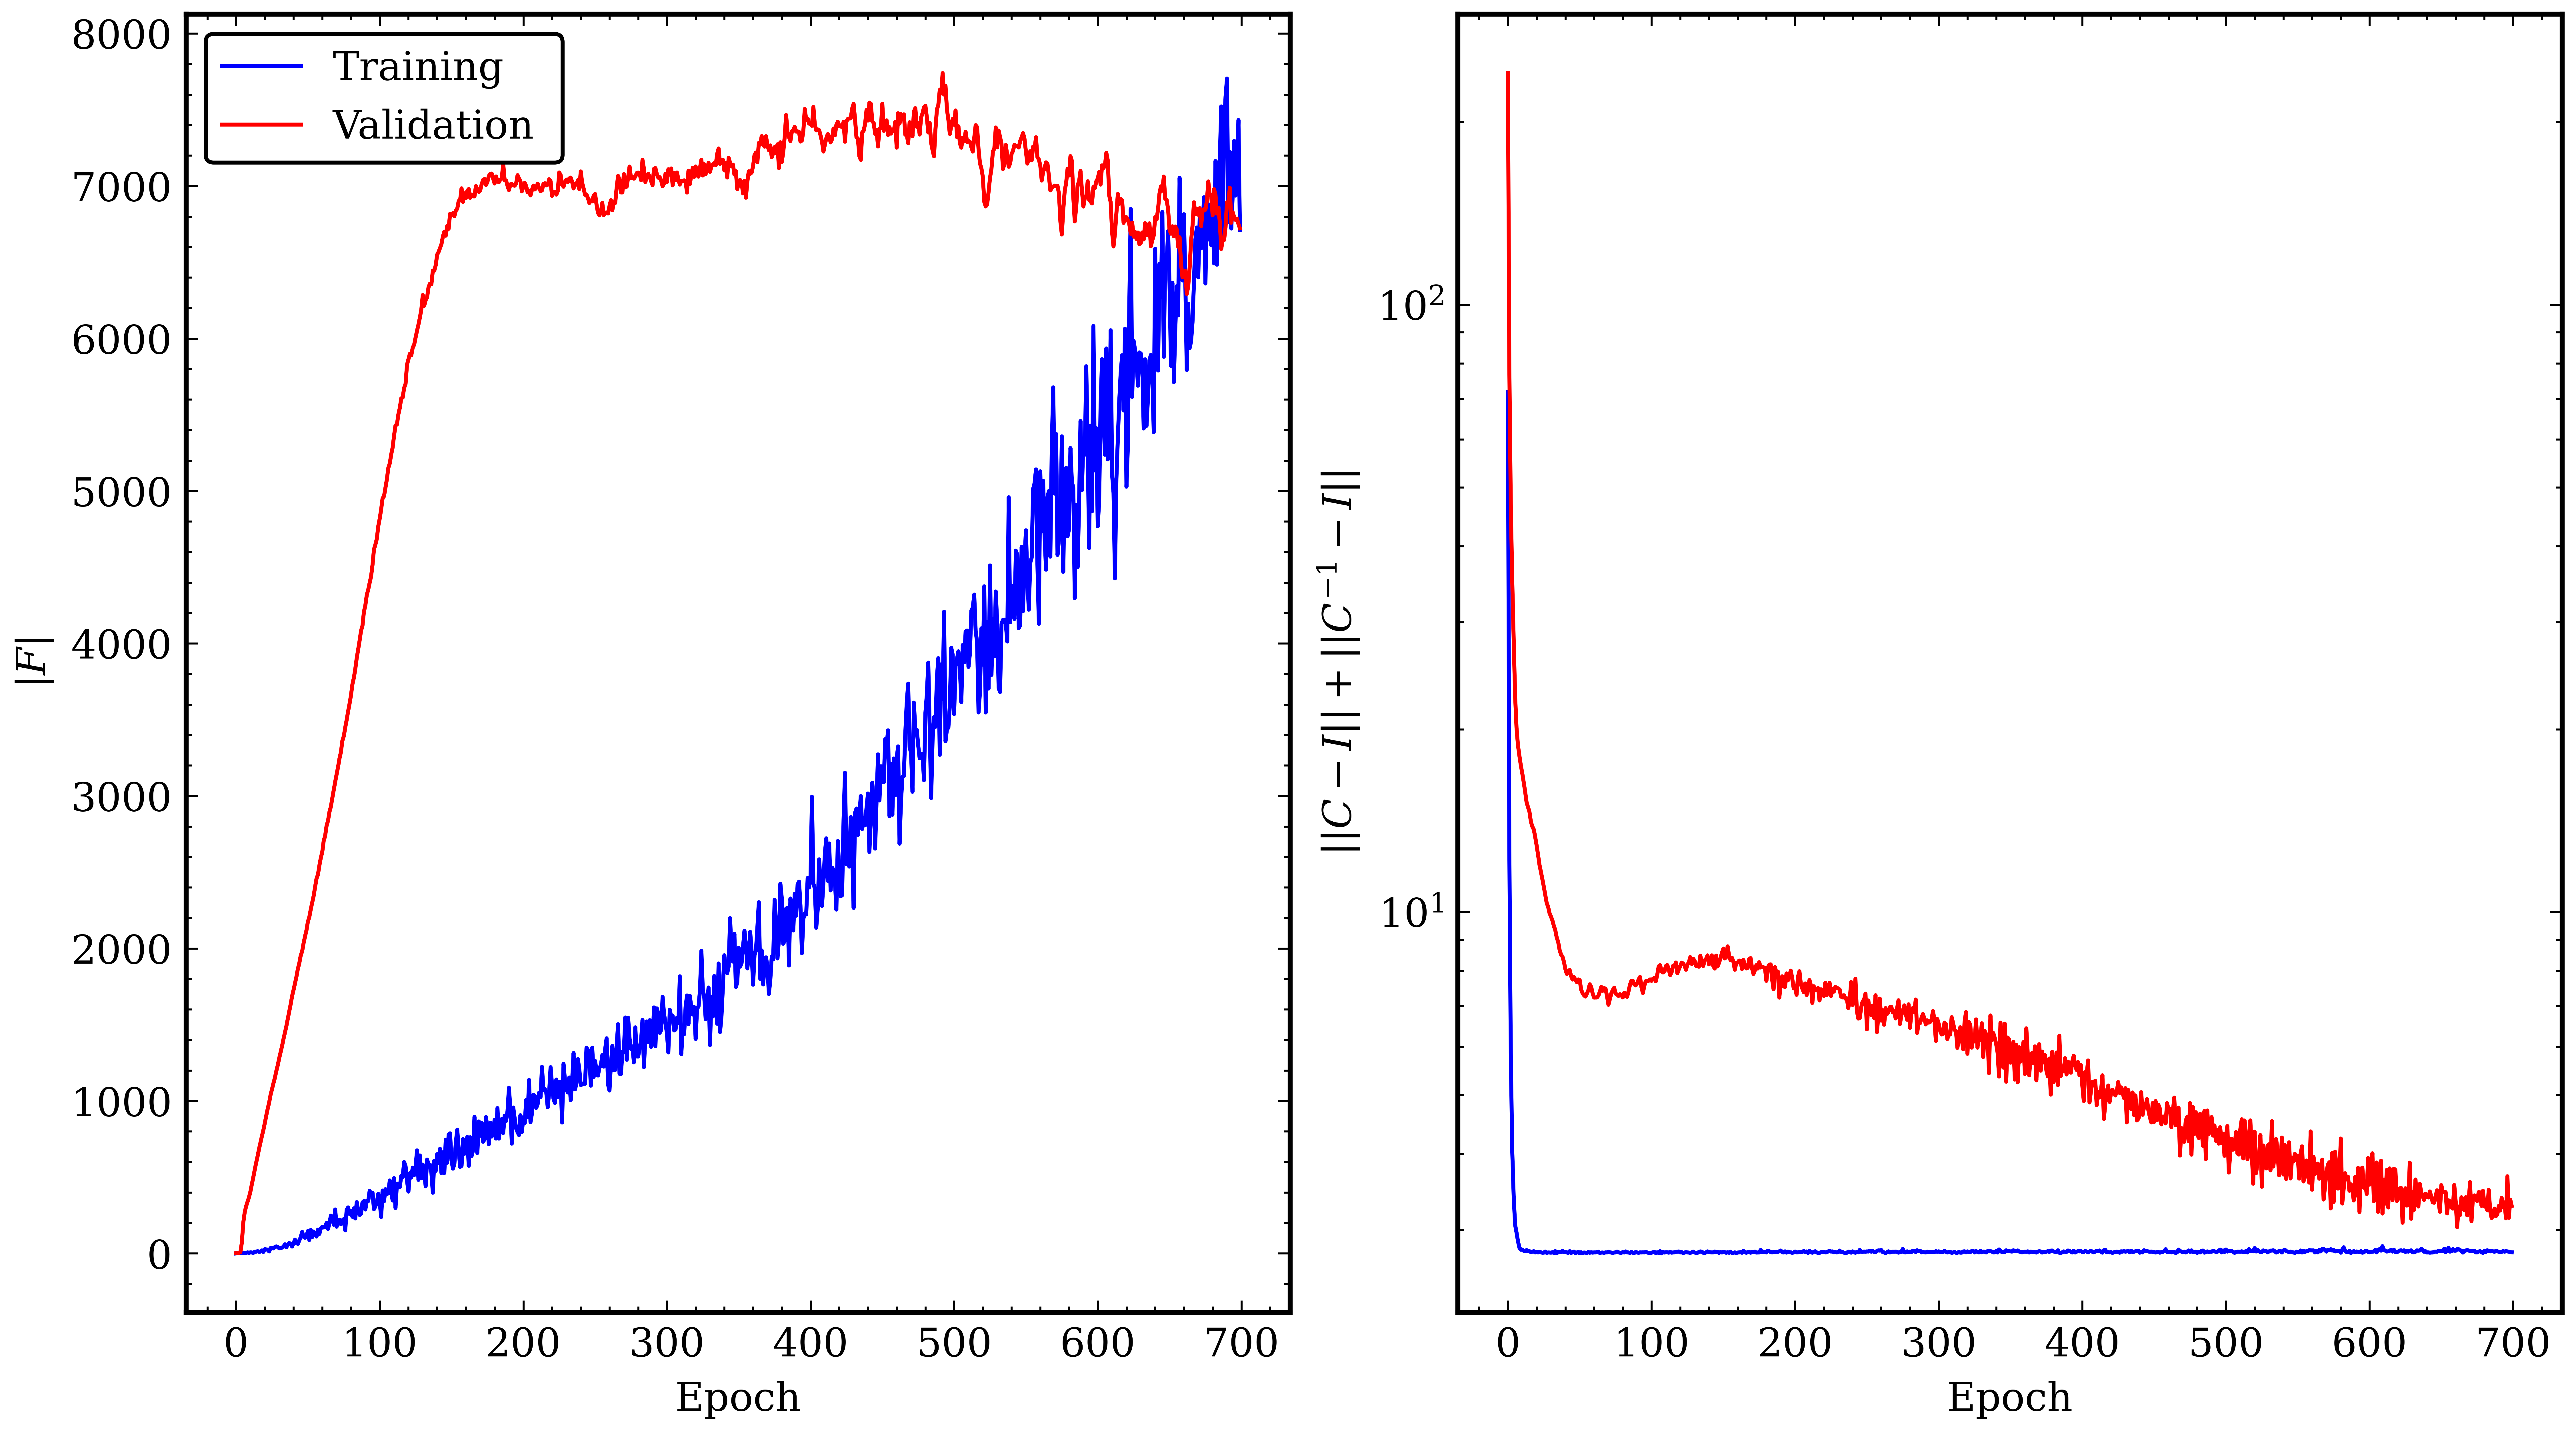
\includegraphics[width=0.95\linewidth]{img/ML/normal_plot_training.png}
    \caption{$|F|$ and $||C-I ||+||C+I||$ as a function of the epoch for the training and validation sets during the training of the IMNN on a normal field. The goal is to find summaries to optimally extract information about the mean and variance of the field.}
    \label{fig:IMNN training normal test}
\end{figure}

To better interpret the network output and to understand its behavior, we generate samples of the same size with the zero mean but a standar deviation randomly sampled from $(0,12)$. We then compute the exact statistic (the sample standar deviation) and plot it against the second IMNN sumamry output. The result is Figure \ref{fig:IMNN normal std}. Observe that the exact statistic in the $x$-axis is highly correlated to the network summary in the $y$-axis. Since the relation between the two quantities is clearly bijective, the model has succesfully learnt to extract all the possible information for the field covariance. The natural scatter is due to having a simple NN model.

\begin{figure}
    \centering
    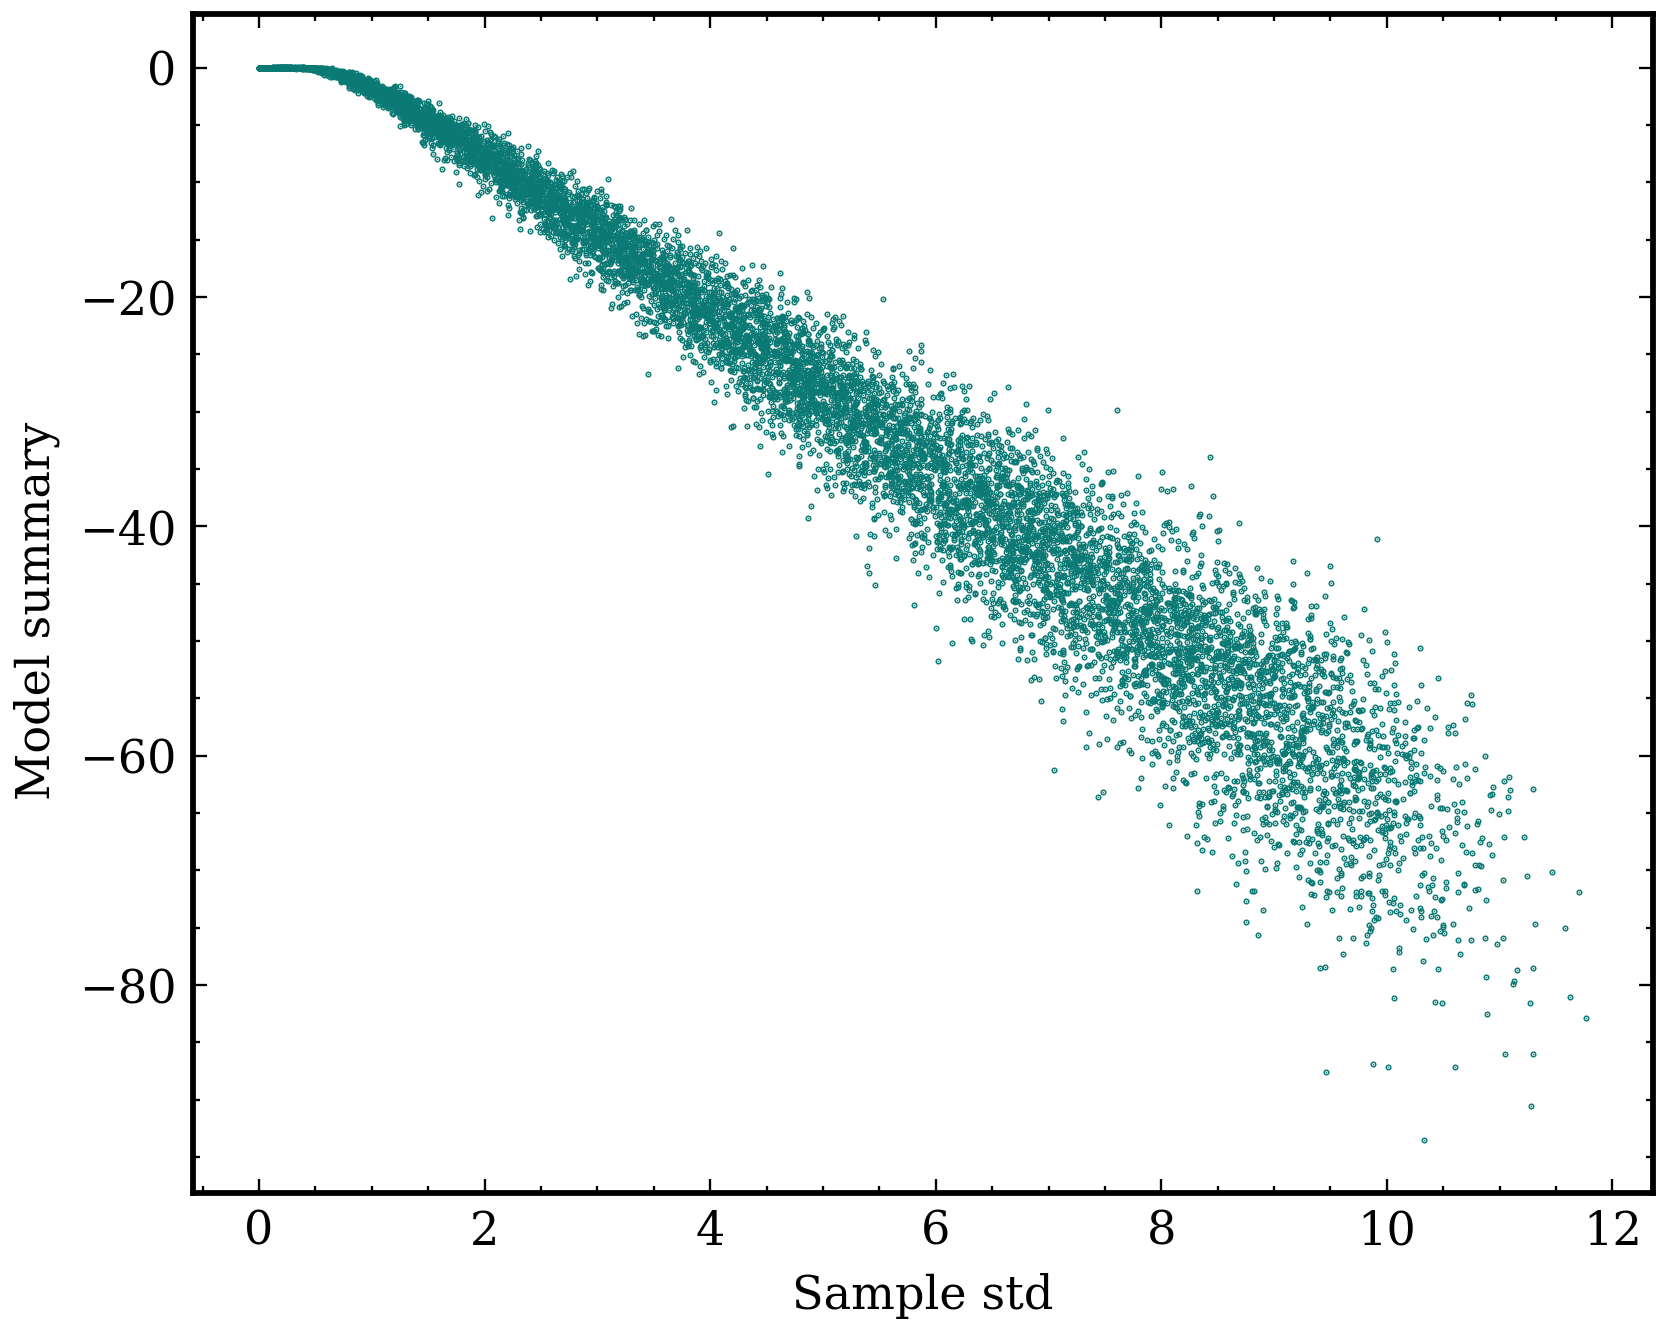
\includegraphics[width=0.75\linewidth]{img/ML/std_vs_model.png}
    \caption{The IMNN summary plotted agains the exact sufficient statistic for the standard deviation using multiple samples with $\sigma \in (0,12)$.}
    \label{fig:IMNN normal std}
\end{figure}
Note that the network has not seen any normal field with such variances $\sigma \in (0,12)$ during training, yet it is able to extract the correct summary. This is of crucial importance, since it means that we could use the IMNN summaries to do inference on a field with parameter values slighly different from the fiducial ones used during training.


To conclude the exploration of this toy model, we use the network to perform Bayesian inference. We implement a simple Approximate Bayesian Computation (ABC) \cite{review_ABC} algorithm that obtains approximate posterior samples from a given set of prior samples and observed data. As the observed data, we take 50 Gaussian fields simulated at fiducial parameter $(\mu=0, \sigma=1)$ values. As priors, we take 5000 samples from a non-informative uniform distribution in $(-5, 5)$ for $\mu$ and $(0, 10)$ for $\sigma$. The ABC rejection algorithm is described in Algorithm \ref{alg:ABC}.


\begin{algorithm}
    \caption{Approximate Bayesian Computation Rejection Algorithm}\label{alg:ABC}
    \begin{algorithmic}[1]
    \State \textbf{Input:} Observed data $\mathbf{y}$, threshold $\epsilon$, number of simulations $N$, prior distribution $\pi(\theta)$
    \State \textbf{Output:} Accepted parameter values $\{\theta_i\}_{i=1}^M$
    
    \State Initialize $M \gets 0$
    \For{$i = 1$ to $N$}
        \State Sample $\theta^*$ from the prior distribution $\pi(\theta)$
        \State Simulate data $\mathbf{y}^*$ from the model using $\theta^*$
        \If{$d(\mathbf{y}, \mathbf{y}^*) \leq \epsilon$}
            \State Accept $\theta^*$: $\theta_{M+1} \gets \theta^*$
            \State Increment $M \gets M + 1$
        \EndIf
    \EndFor
    
    \State \textbf{return} $\{\theta_i\}_{i=1}^M$
    \end{algorithmic}
    \end{algorithm}
In Figure \ref{fig:IMNN normal posterior} we show the posterior samples and Gaussian Kernel Density Estimation (KDE) for the distributions of $\mu$ and $\sigma$. The dashed vertical lines show the true parameter values. As expected, and even with a non-informative prior, the IMNN summary contain sufficient information to produce tight posterior around the true model parameters. Note that the posterior scatter on the non-linear summary $\sigma$ is larger than on the linear summary $\mu$.

\begin{figure}
    \centering
    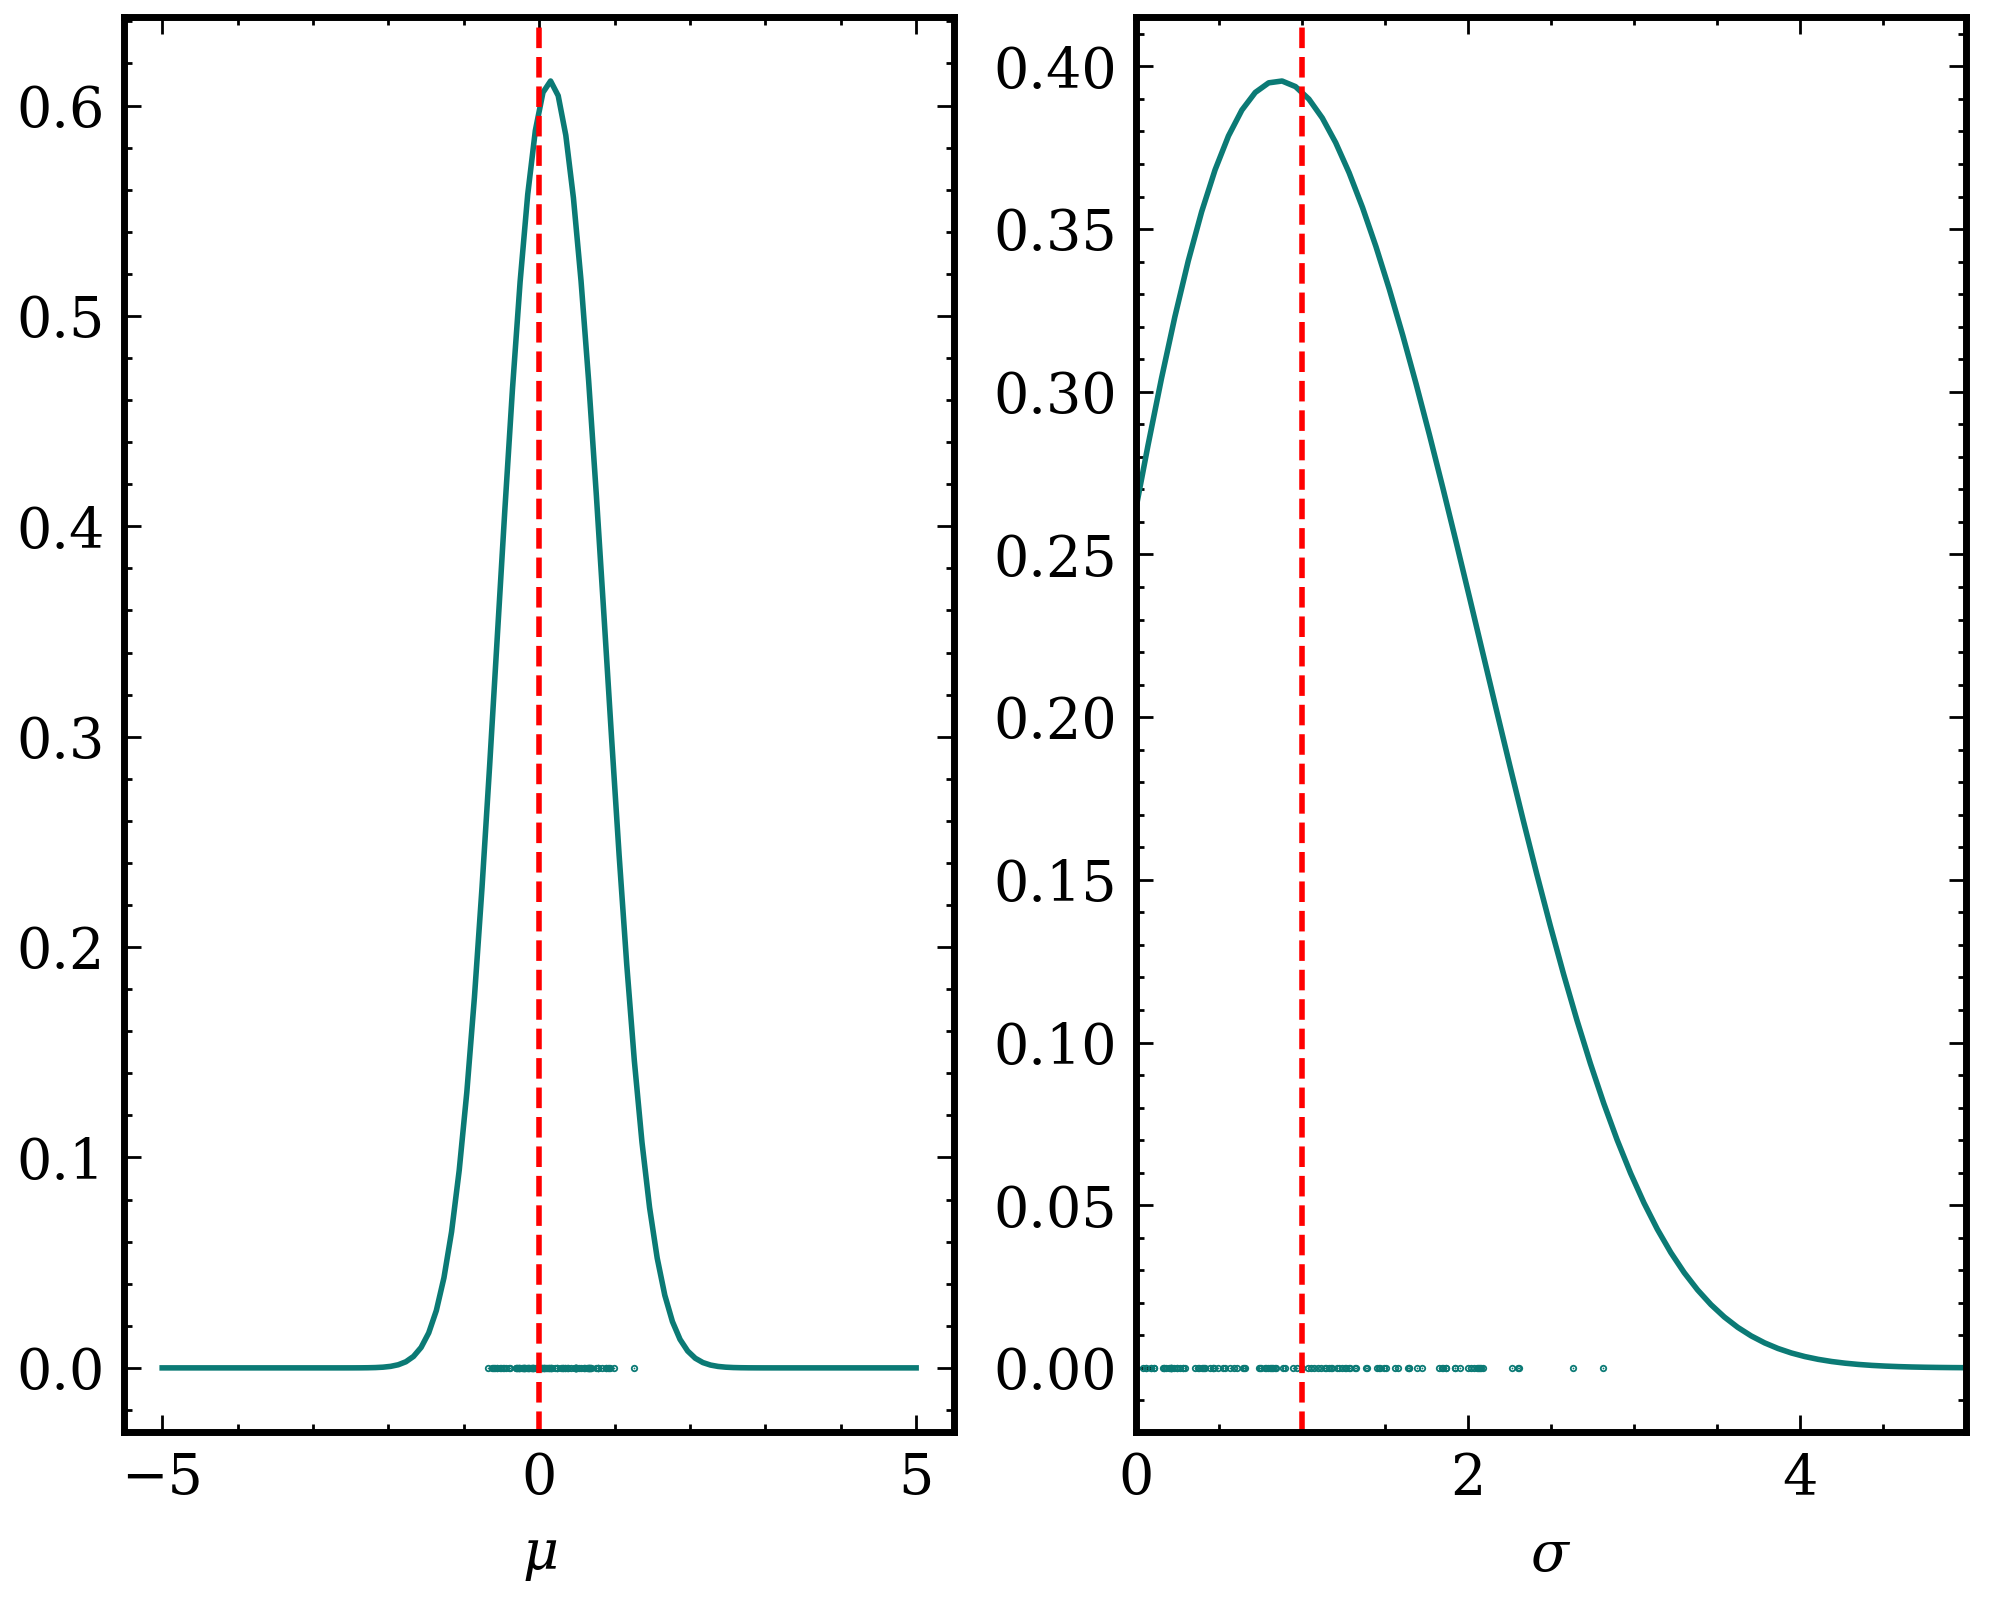
\includegraphics[width=0.75\linewidth]{img/ML/ABC_posteriors_normal.png}
    \caption{Posterior samples and KDE for the ABC rejection algorithm applied to the normal toy model, where we infer the mean and variance of a Gaussian field with flat priors and the summaries output of a IMNN. The dashed vertical lines show the true parameter values.}
    \label{fig:IMNN normal posterior}
\end{figure}






\subsection{IMNN inference results on WDM masses}\label{sec:IMNN}
We can now deploy a simple IMNN as an alternative way of constraining WDM models. We follow section \ref{sec:IMNN normal} and consider a similar architecture but now with 4 dense layers of size $[512, 512, 256, 2]$. As input to the NN, we consider Lyman-$\alpha$ flux skewers. Since in flux space the skewers has many simulation-specific and prominnent features that can be picked-up by a NN, we work in Fourier space. More precisely, the input to the network are 
\begin{equation}
    \sqrt{k} |\delta_F (k)|,
\end{equation}
where $\delta_F$ is the flux contrast of the skewer.
We use the \texttt{SHERWOOD} simulation suite with varied WDM mass to train the IMNN. Note that this means that we are assuming that WDM is the only model parameter affecting the Lyman-$\alpha$ forest property. We ignore thermal parameters variations for this demosntration. We train our model on the fiducial CDM mass corresponding to $0$ Kev$^{-1}$, and use the WDM3 model corresponding to $0$ Kev$^{-1}$ to calculate the summary derivatives. The choice of WDM3 is due to the flux skewers showing sufficient variation with respect to CDM.

\begin{figure}
    \centering
    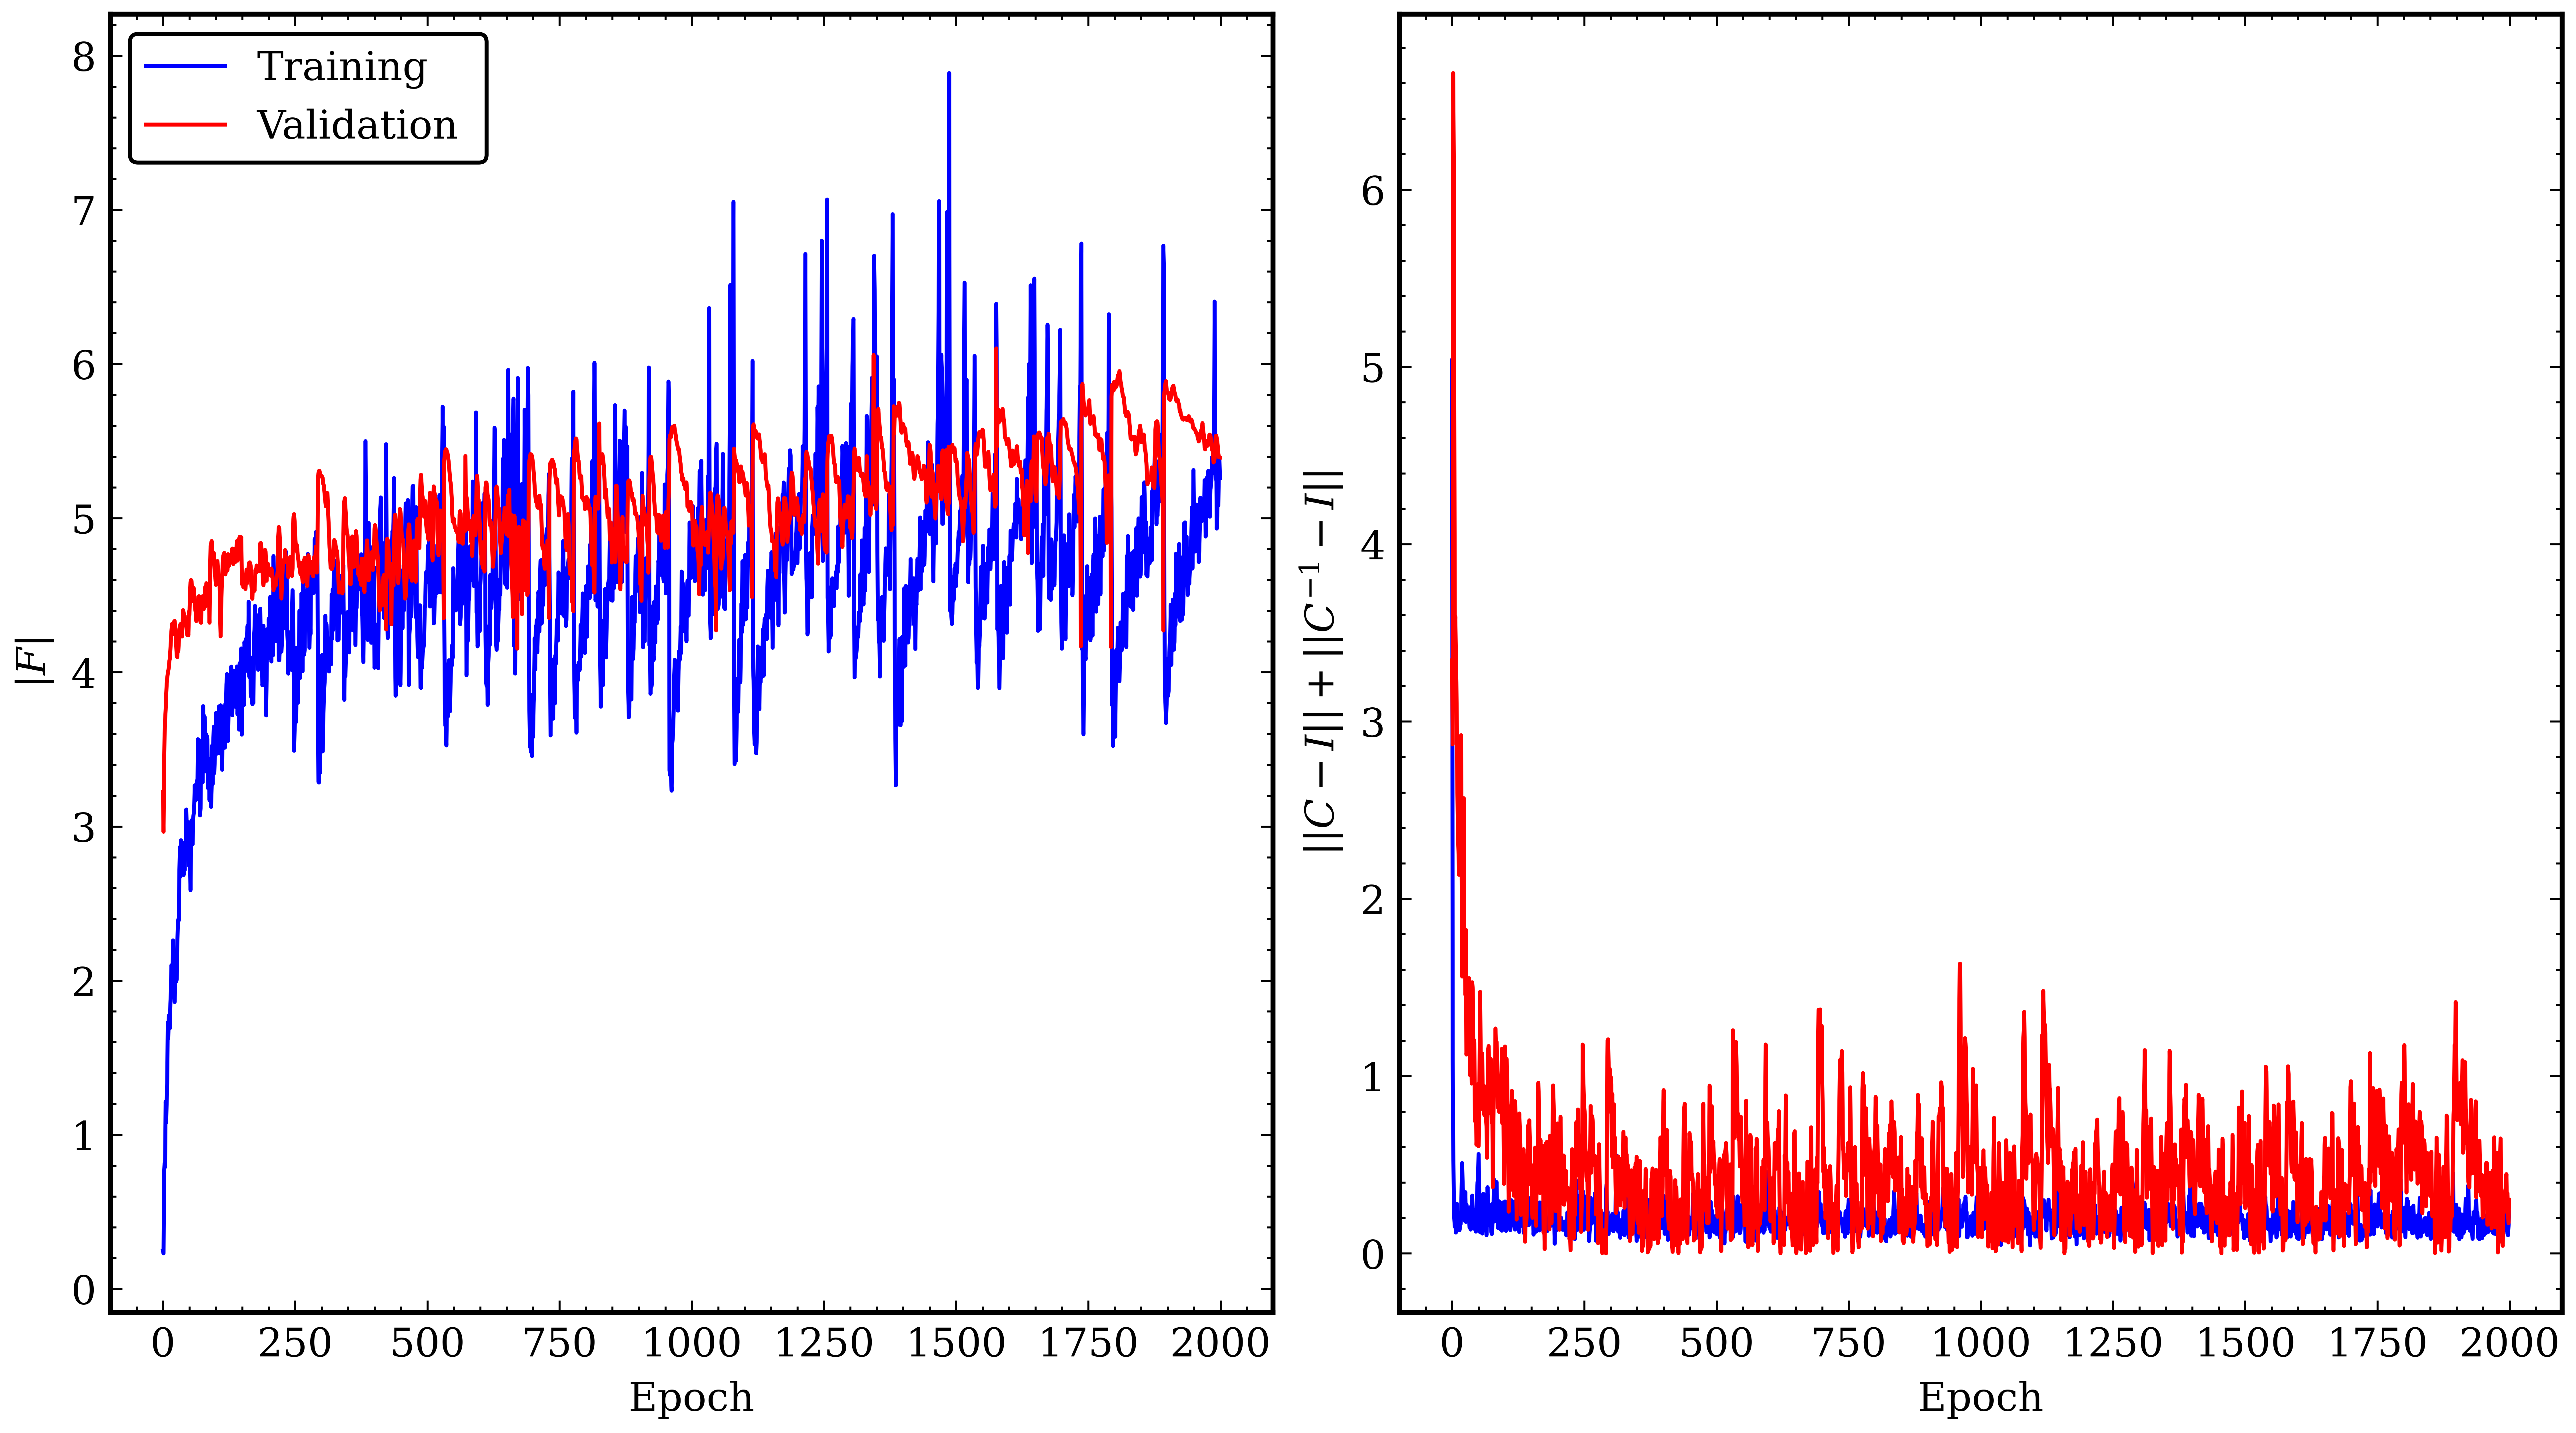
\includegraphics[width=0.95\linewidth]{img/ML/WDM_training_plot.png}
    \caption{$|F|$ and $||C-I ||+||C+I||$ as a function of the epoch for the training and validation sets during the training of the IMNN on the \texttt{SHERWOOD} dataset Lyman-$\alpha$ skewers.}
    \label{fig:IMNN  wdm training}
\end{figure}
In Figure \ref{fig:IMNN wdm training} we show the training progress of the IMNN as a function of the epoch. The information extracted on the validation split quickly saturates at $\sim 250$ epochs. It is clear that the network is able to learn a map from Lyman-$\alpha$ skewers in Fourier space into a one-dimensional parameter space. Since the \texttt{SHERWOOD} suite has a fix number of simulations, interpreting the network output summaries is a challenging task.


\begin{figure}
    \centering
    \begin{subfigure}[b]{0.53\textwidth}
        \centering
            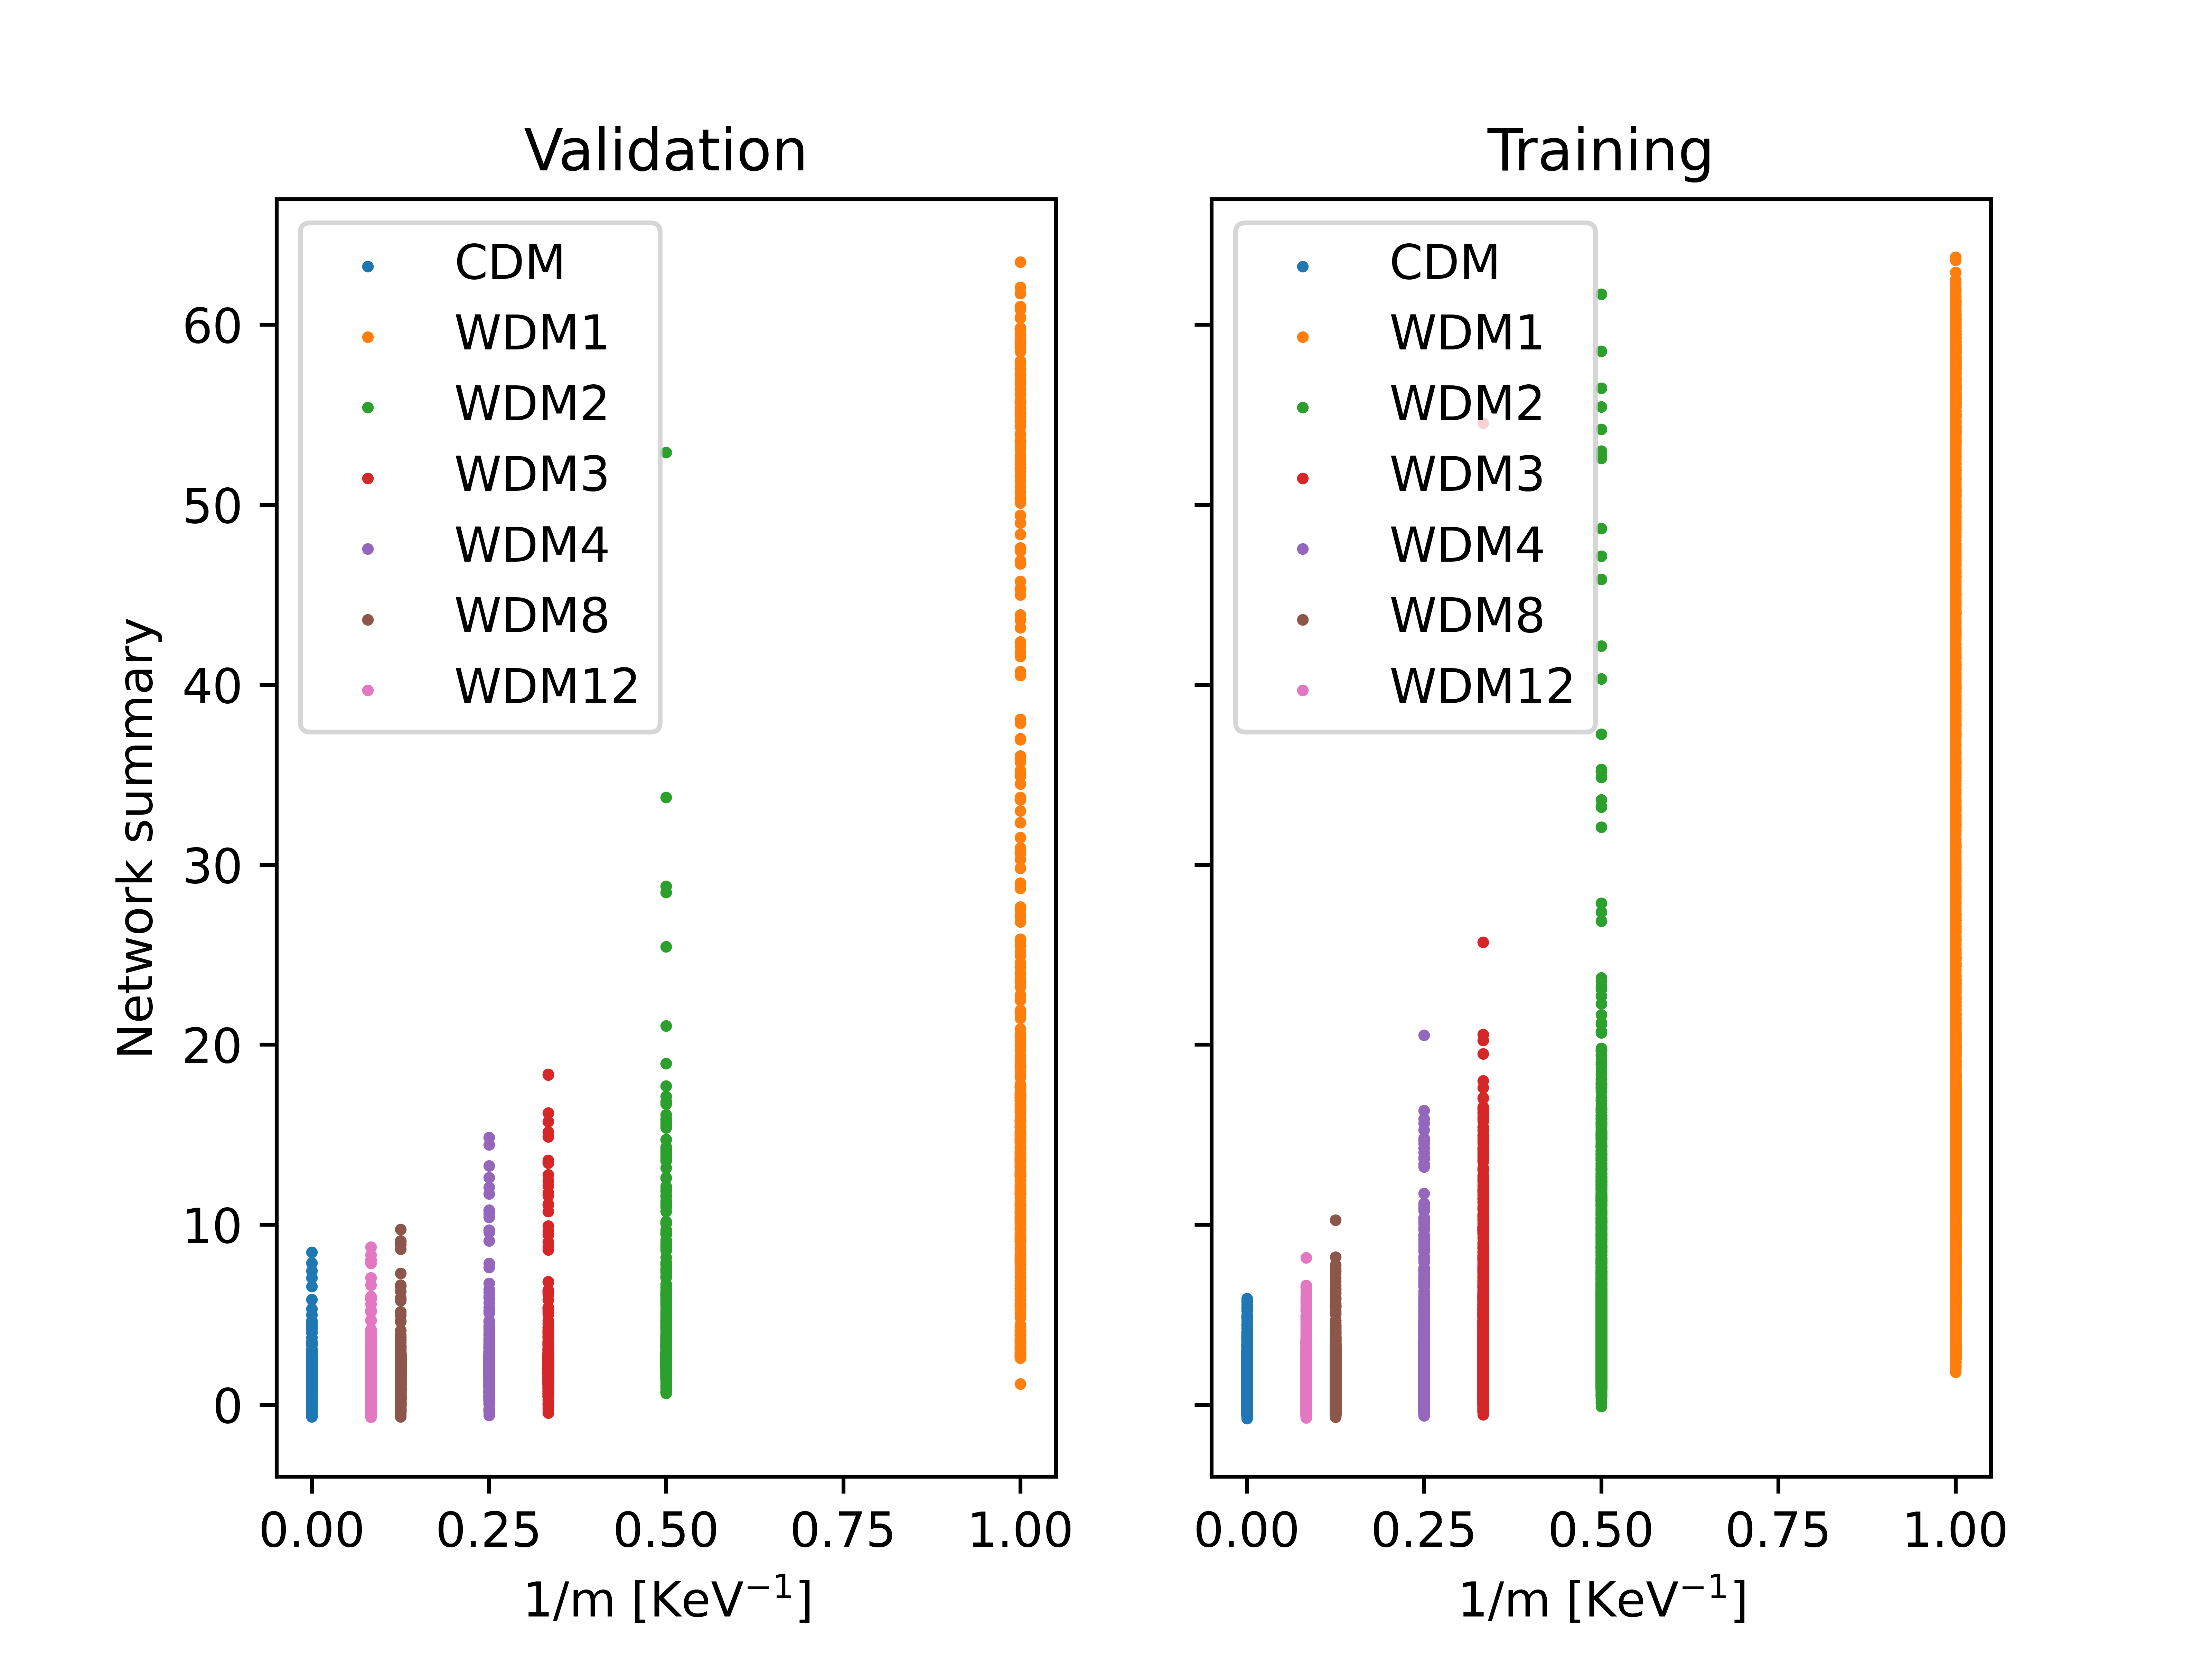
\includegraphics[width=1\textwidth]{img/ML/IMNN_output.png}
            \caption{IMNN outputs for the \texttt{SHERWOOD} Lyman-$\alpha$ skewers.}
    \end{subfigure}
    \hfill
    \begin{subfigure}[b]{0.45\textwidth}
        \centering
        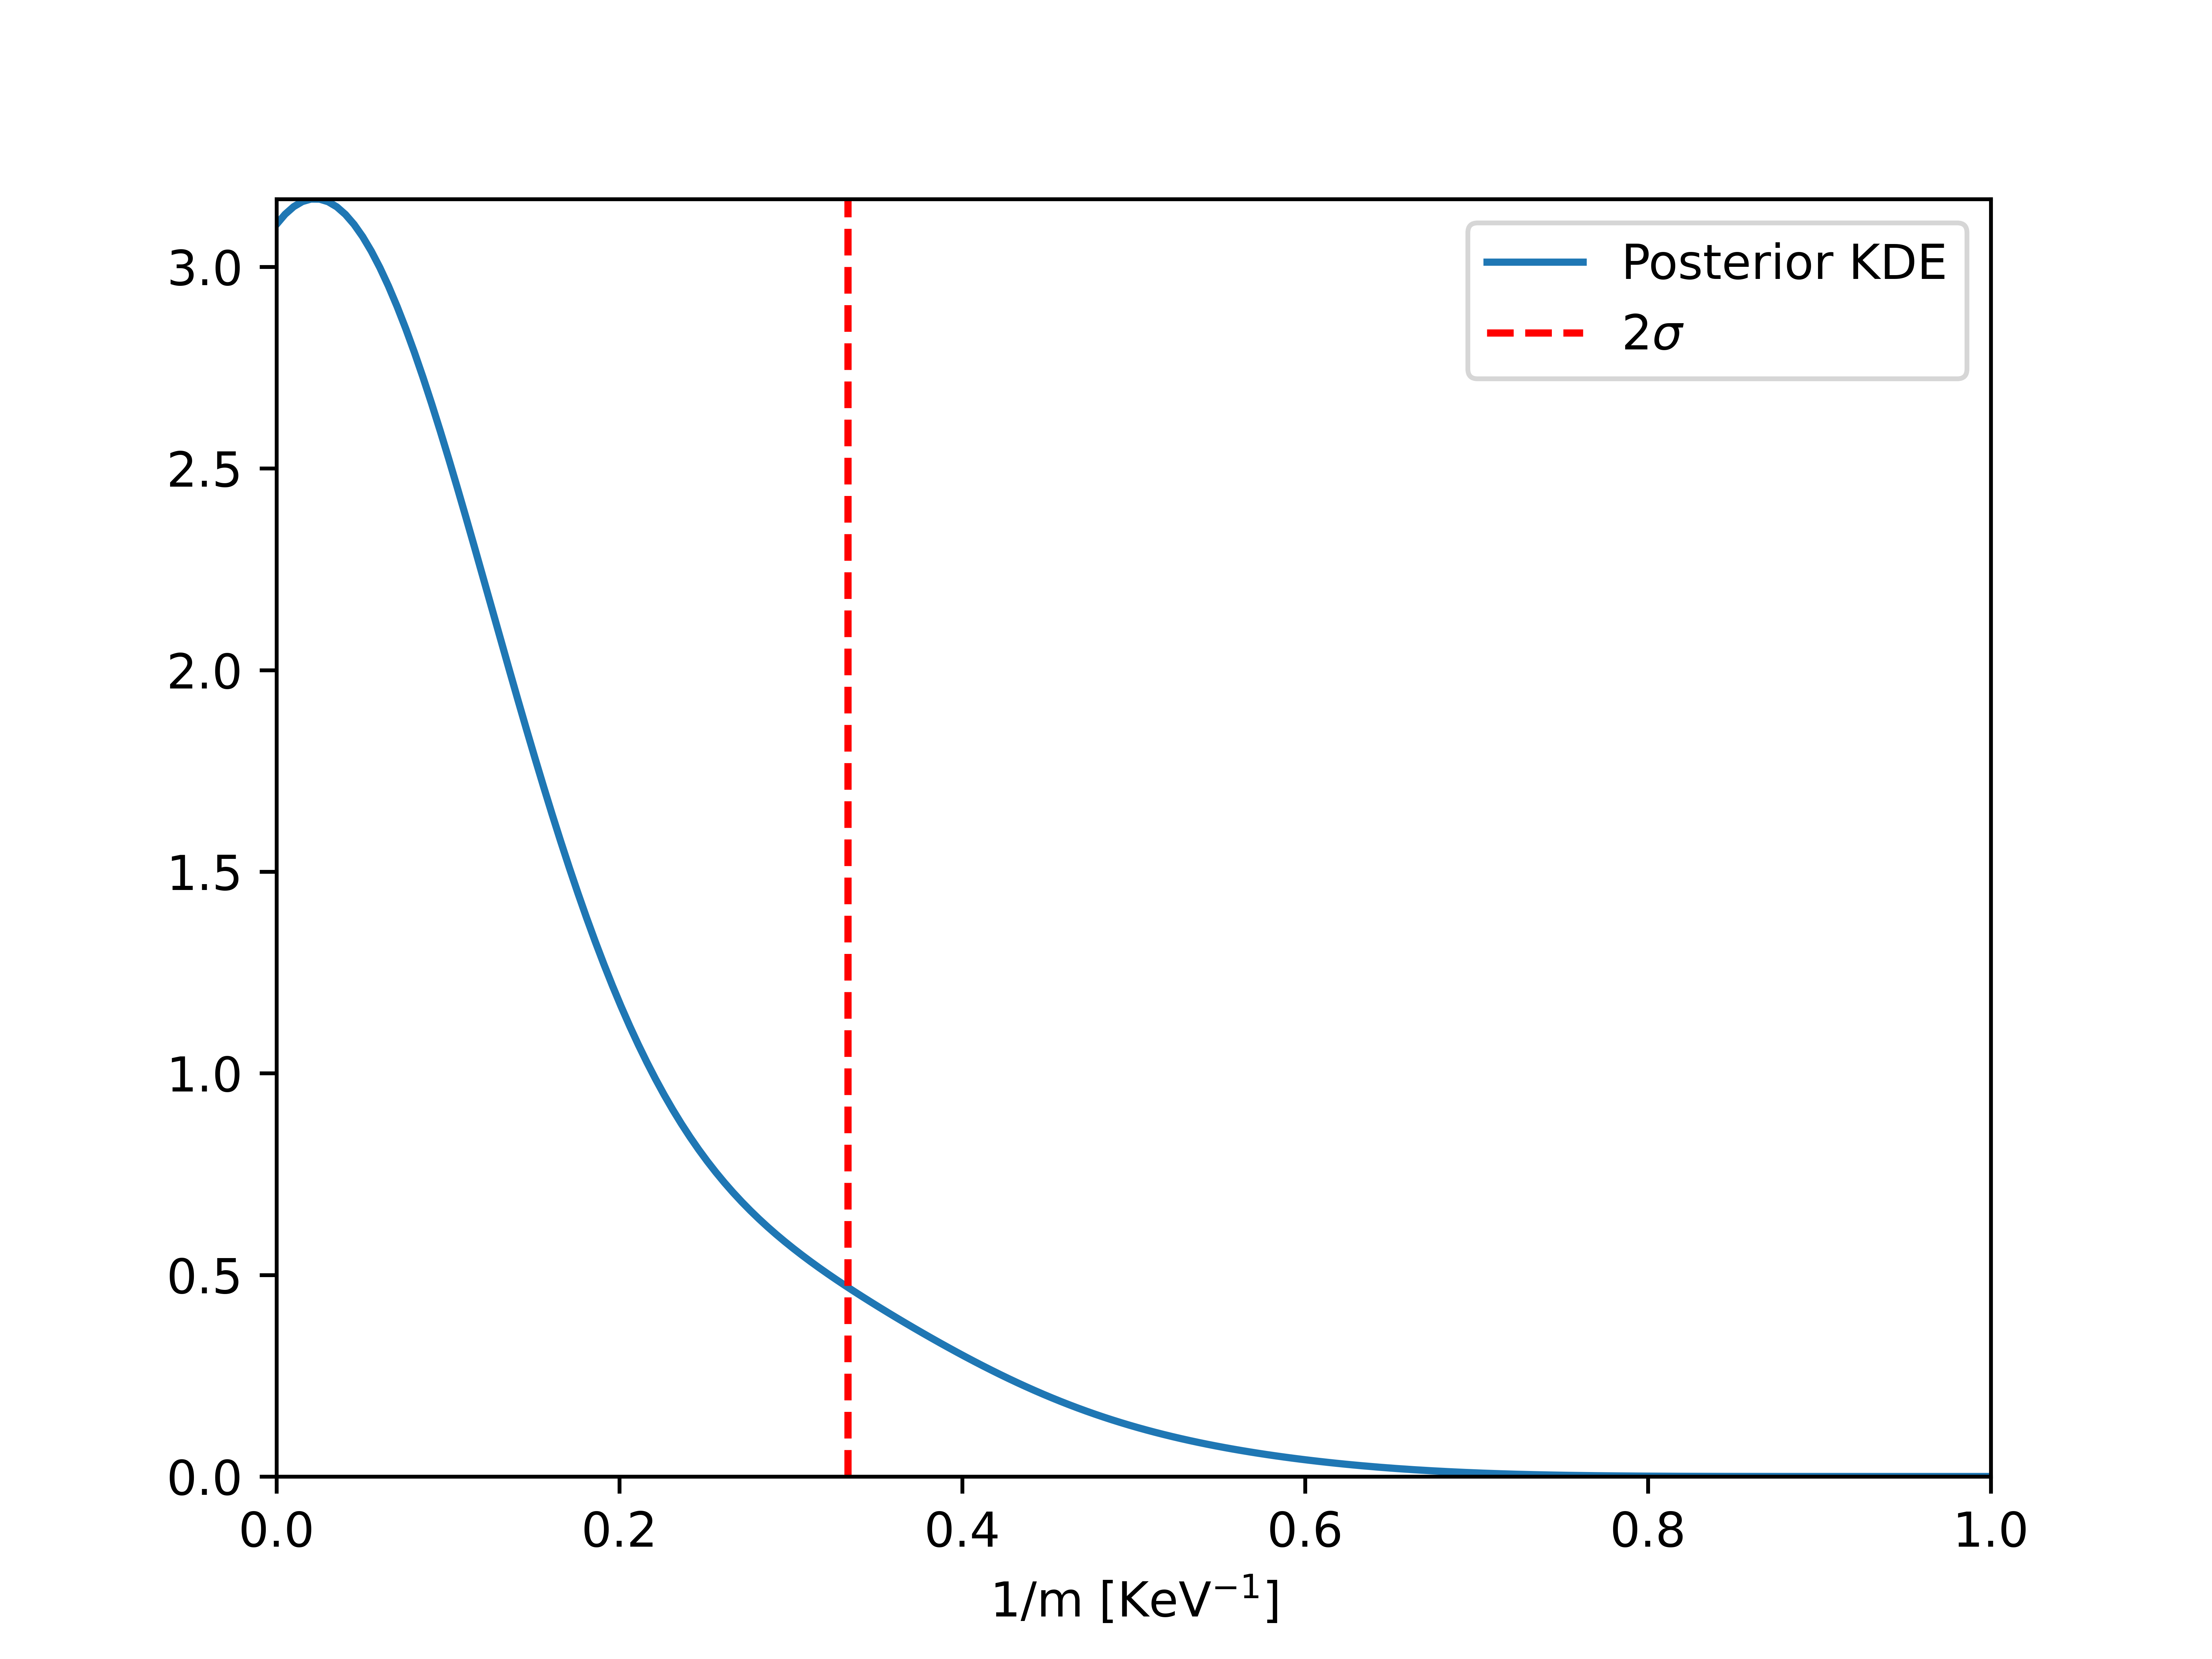
\includegraphics[width=1\textwidth]{img/ML/IMNN_ABC_wdm.png}
        \caption{ABC WDM mass posterior for a test of 50 observed CDM skewers. The $2\sigma$ WDM constraint is $\sim 3 $ Kev.}     
    \end{subfigure}
        \caption{}
        \label{fig:IMNN WDM posterior}
\end{figure}

In Figure \ref{fig:IMNN WDM posterior}a) we show the summaries of the trained IMNN for all the aviable \texttt{SHERWOOD} Lyman-$\alpha$ skewers is Fourier space. Observe how the summaries show a large scatter for every model, corresponding to the large simulation variability within each skewer. However, the mean summaries show a clear bijective trend, manifesting that the IMNN has learnt an informative summary. Note that this can be interpreted as the necessity of a large number of observed samples when constraining WDM models.
We use the IMNN summaries to perform an inference test and obtain a Bayesian posterior as follows. First, we select 50 CDM skewers from the validation dataset and obtain their corresponding summaries by passing them through the IMNN. We now use all validation skewers from the \texttt{SHERWOOD} suite and obtain their summaries. We use the ABC rejection algorithm \ref{alg:ABC} to generate to posterior distribution in Figure \ref{fig:IMNN WDM posterior}b). The $2\sigma$ limit for the WDM mass is $\sim 3$ KeV. Recall that this is a comparable constraint to the one obtained in section \ref{sec:inference squad}. We interpret this not only as a robustness sign of our original pipeline involving a $\chi^2$ fit the $\Delta_\tau$ PDFs, but most notably as a sign that it optimally extracts the majority of the information of the Lyman-$\alpha$ skewers with respect to the WDM mass parameter.

























